The main topic of this thesis is Partially Observable Markov Decision Processes (POMDPs).
The practical use of this model has been criticized in Introduction, 
however it sums up accurately the principal features of a robotic system.
As we ambition to make this thesis mathematically self-contained
the POMDP model is built in Section \ref{section_Markov2POMDP} 
from low level objects of Probability Theory.
The main ways to compute strategies from this model are then summarized
in Section \ref{section_SAalgo}.
Next, Possibility Theory is presented
in order to introduce Qualitative Possibilistic Markov Decision Processes ($\pi$-MDPs)
and Partially Observable ones ($\pi$-POMDPs) which are the starting point
of this work.

\section{From Markov Chains to Partially Observable Markov Decision Processes}
\label{section_Markov2POMDP}
The first theoretical object behind the POMDP model, 
as its name suggests, 
is the \textit{Markov Chain}. 
In order to present it, let us look back one century ago.
\subsection{Markov Chains}
\label{section_MarkovChains}
In the early years of the twentieth century Andre\"i Markov,
a doctoral student of Pafnouti Tchebychev, 
set up Markov Chains. 
Studying successive letters in the words of novels,
he had the idea to define this kind of sequence of random variables:
indeed, each letter depended primarily on the previous one. 
As usual, a random variable 
is a measurable function defined 
on a set $\Omega$ equipped with a $\sigma$-algebra $\mathcal{F}$
and a probability measure $\mathbb{P}$. 
\begin{Def}[Markov Chain]
\label{def_markov_chain}
Let $\mathcal{S}$ be a countable set called \textit{set of states}
and $(S_t)_{t \in \mathbb{N}}$ a sequence of random variables
whose values are in $\mathcal{S}$. The sequence $(S_t)_{t \in \mathbb{N}}$ 
is a Markov Chain if $\forall t \geqslant 1,  \forall (s_0,s_1,\ldots,s_{t+1}) \in \mathcal{S}^{t+2}$
\begin{equation}
\label{eq_markov_property}
\mathbb{P} \paren{ S_{t+1} = s_{t+1} \sachant S_0 = s_0,S_1=s_1, \ldots, S_t=s_t} 
= \mathbb{P} \paren{ S_{t+1} = s_{t+1} \sachant S_t = s_{t} }
\end{equation}
\textit{i.e.} $\forall t \geqslant 1$,
the random variable $S_{t+1}$ 
is independent from all previous variables 
$\set{ S_i \sachant i \leqslant t-1 }$
conditional on the random variable $S_t$:
the value of $S_0$, or its probability distribution is given, and
the probability distribution of $S_{t+1}$ only depends on 
the value of $S_t$ and on the time step $t \geqslant 0$ 
(see Figure \ref{fig_markov_chain}).
\end{Def}
Figure \ref{fig_markov_chain} describes 
the Bayesian Network \cite{Pearl:1988:PRI:52121,pearl85bayesian} of a Markov Chain.
In a Bayesian Network, or directed acyclic graphical model, 
the variables are represented by nodes. 
The absence of an arrow between two random variables (nodes) 
represents an assumption about the conditional independence of the variables.
Let $S'$ be a random variable: 
the set of variables from which an arrow starts 
and leads to $S'$ is called the set of \textit{parents} of $S'$, 
and denoted by $parents(S') = \set{ S \sachant S \rightarrow S' }$.
If $S \in parents(S')$, we say that $S'$ is a \textit{children} of $S$: 
the set of the children of $S$ is denoted by $children(S)$.
The set of the \textit{descendants} of a random variable $S$ 
is the smallest set of variables $descend(S)$
which contains all the children of $S$ 
and such that $\forall S' \in descend(S)$, $children(S') \subset descend(S)$ 
\textit{i.e.} all the children of a descendant is a descendant.
The assumption taken through a Bayesian Network is that each variable $S$ 
is independent from its \textit{non-descendants} 
$nondescend(S) = \set{\tilde{S} \notin descend(S) \cup \set{ S } \cup parents(S) }$
conditional on its parents $parents(S)$,
denoted by: 
\[ S \perp\!\!\!\perp nondescend(S) \hspace{0.2cm} \vert \hspace{0.2cm} parents(S). \]
In other words, $S$ only depends on its direct parents. 
Figure \ref{fig_markov_chain} is also called Dynamic Bayesian Networks (DBNs) 
\cite{Dean:1989:DBN} since the arrows model also successive time steps. 


Here, the \textit{Markov Property} \textit{i.e.} 
Equation \ref{eq_markov_property} of Definition \ref{def_markov_chain},
implies that $\forall t \in \mathbb{N}$,
the variable $S_{t+1}$
has only one arrow pointing to it
from $S_t$
\textit{i.e.} 
the variable $S_{t+1}$ has only one parent
in the Network, which is $S_{t}$.
\begin{figure}
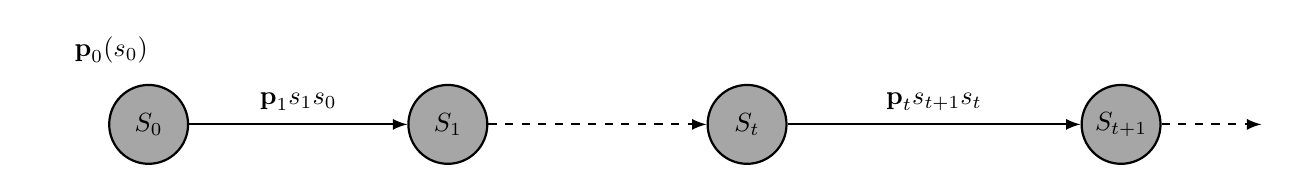
\begin{tikzpicture}[transform shape,scale=0.95]
% vertex shape and color
\tikzstyle{vertex}=[circle,fill=black!35,minimum size=30pt,inner sep=0pt, draw=black,thick]

% nodes
\node (left) at (-1.5,0) {};
\foreach \name/\x in {S_0/0,S_1/4,S_t/8, S_{t+1}/13}
\node[vertex] (G-\name) at (\x,0) {$\name$};
\node (G-end) at (15,0) {};

% arrows
\foreach \from/\to in {S_0/S_1,S_t/S_{t+1}}
\draw[->,>=latex,thick] (G-\from) -- (G-\to);
\foreach \from/\to in {S_1/S_t,S_{t+1}/end}
\draw[->,>=latex,dashed,thick] (G-\from) -- (G-\to);

% transition probabilities
\node (proba0) at (-0.5,1) {$\textbf{p}_0(s_0)$};
\node (proba1) at (2,0.3) {$\textbf{p}_1 \paren{ s_{1} \sachant s_{0}}$};
\node (probat) at (10.5,0.3) {$\textbf{p}_t \paren{ s_{t+1} \sachant s_{t}}$};
\end{tikzpicture}

\caption[Bayesian Network of a Markov Chain]{Bayesian Network of a Markov Chain:
each node (black circle) represents a random variable. 
Each variable $S_{t+1}$ has only one parent $S_t$: $\forall t\geqslant1$
$S_{t+1} \perp\!\!\!\perp \set{ S_{0}, \ldots, S_{t-1} } \vert S_t$.}
\label{fig_markov_chain}
\end{figure}

As $\mathcal{S}$ is countable, 
let us number its elements, the \textit{states}: 
$\mathcal{S}=\set{ s^{(1)},s^{(2)}, \ldots}$. 
The probabilistic dynamics of a Markov Chain 
can be represented by 
a sequence of stochastic matrices\footnote{A stochastic matrix
is a matrix whose values are non-negative real numbers and whose rows sum to one.} 
$(M_{t})_{t \in \mathbb{N}}$ 
defined by $ (M_t)_{i,j} = \mathbb{P} \paren{ S_{t+1}=s^{(j)} \sachant S_{t} = s^{(i)}}$.
Note that the model is entirely defined 
given this sequence of matrices 
and the distribution of the first random variable $S_0$:
$\textbf{p}_0(s) = \mathbb{P}(S_0=s)$.
For a better readability, $\mathbb{P} \paren{ S_{t+1}=s' \sachant S_{t} = s}$ 
is denoted by $\textbf{p}_t \paren{s' \sachant s}$,
and called the 	\textit{transition probability distribution}.

An important result about the Markov Chains is the following:
\begin{Property} \label{res_markov}
Let $(S_t)_{t \in \mathbb{N}}$ be a Markov Chain 
whose values are in the countable set of states $\mathcal{S}$.\\ 
$\forall t \in \mathbb{N}$, $\forall f: \mathcal{S} \rightarrow \mathbb{R}$ bounded, 
$\forall (s_0,\ldots,s_{t}) \in \mathcal{S}^{t+1}$,
\begin{align*}
\mathbb{E} \croch{ f(S_{t+1}) \sachant S_0 = s_0, \ldots, S_t = s_t }  
&= \sum_{s' \in \mathcal{S}} f(s') \cdot \mathbb{P} \paren{ S_{t+1} = s' \sachant S_t = s_t } \\
&= \mathbb{E} \croch{ f(S_{t+1}) \sachant S_t = s_t }.
\end{align*}
\end{Property}
The proof is given in Annex \ref{res_markov_RETURN}.

This result will help rigorously set up Markov Decision Processes,
presented in the next section.

\subsection{Markov Decision Processes}
\label{subsection_MDP}
MDPs \cite{puterman94} were proposed
was built to model \textit{systems} 
subject to a probabilistic uncertainty
dependent on \textit{actions} over \textit{time}.
In its classical formulation, the finite set $\mathcal{S}$
defines the possible \textit{states of the system} $s \in \mathcal{S}$.
Here, for the needs of 
the POMDP model building 
in a following section,
$\mathcal{S}$ is defined as a countable set of states, 
as stated earlier.
The set of the non-negative integers $\mathbb{N}$ 
models the \textit{time},
or \textit{stages of the process}.
Possible \textit{actions}, denoted by $a$, 
are chosen from a finite set $\mathcal{A}$.
In order to get a clear overview 
of what information is used 
to decide each action, 
the \textit{agent} is defined as
the entity responsible for decision making,
\textit{i.e.} she/he must choose the successive actions
given the informations about the system.
In our case, a system state $s \in \mathcal{S}$ 
consists of the features of both a robot 
and its environment,
needed to describe the robotic mission.
The agent is in this case 
the decision making part of the robot
who determines the robot's actions
to be exectuted 
given the successive states of the system.

If the sequence of chosen actions $a \in \mathcal{A}$
is known, an MDP is a Markov Chain:
the system state of an MDP at stage $t+1$,
represented by the variable $S_{t+1}$,
only depends, in the probabilistic meaning of the term,
on the previous system state variable $S_t$
and on the time step $t\geqslant 0$.
However, the agent influences the probabilistic system dynamics
by selecting the actions $a \in \mathcal{A}$ 
at each time step $t \in \mathbb{N}$.

In the MDP framework, it is assumed that 
the agent is perfectly informed 
of the current system state $s_t \in \mathcal{S}$
at each time step. 
Its decision can then be \textit{a priori} 
based on the current system state 
and all previous ones:
Theorem \ref{thm_mdp_finiteH}
shows however that, 
for the used criterion,
it is equivalent to consider 
that each decision is taken
based on the current state only.
A stochastic matrix $M^{d}$ can be defined for
each \textit{decision rule} $\left \{ \begin{array}{ccc}
d : & \mathcal{S} \rightarrow & \mathcal{A} \\
& s \mapsto & d(s)
 \end{array} \right.$ describing transition probability distributions  
of the Markov Chain $(S_t)_{t \in \mathbb{N}}$
if the decision rule $d$ is used: 
$\paren{M^{d}}_{i,j}$ is the probability of reaching the state $s^{(j)}$ from $s^{(i)}$  
when the action $d(s^{(i)})$ is selected by the agent. 
Consider a sequence of decision rules
$(d_t)_{t \in \mathbb{N}}$: 
such a sequence is called \textit{strategy} 
and defines a sequence of stochastic matrices 
$(M_t)_{t \in \mathbb{N}}$ 
with $M_t=M^{d_t}$. 
Each strategy thus defines the parameters of a Markov Chain entirely. 

A reward $r_t(s,a) \in \mathbb{R}$ is associated 
to each triple $(s,a,t) \in \mathcal{S} \times \mathcal{A} \times \set{ 0, \ldots, H-1 }$
to model the importance of going through the state $s$
and selecting action $a$ at time $t$.
The function $r: \mathcal{S} \times \mathcal{A} \times \set{ 0, \ldots, H-1 } \rightarrow \mathbb{R}$
is assumed to be bounded:
this assumption is not necessary if 
$\mathcal{S}$ is finite, as 
$r_t(s,a) \leqslant \displaystyle \max_{s' \in \mathcal{S}}  \max_{ a' \in \mathcal{A}} \max_{ 0 \leqslant t' \leqslant H-1} \set{ r_{t'}(s',a')}$,
however, $\mathcal{S}$ is here countable 
and thus may be infinite.
The value of a system finishing in state $s$
is described by the terminal reward $R(s)$, 
defined for each state $s$. The function $R$
is assumed to be bounded on $\mathcal{S}$.

For instance in the Navigation problem 
of the International Probabilistic Planning Competition,
\cite{SannerIPPC1111}, a robot in a grid has to reach a goal:
if the state $s$ encodes a robot location which is not the goal,
$r_t(s,a)=-1$, and $r_t(s,a)=0$ otherwise.
If the designers of the model want
the robot to be in a sleep mode
at the end of the mission,
terminal reward could have been defined
as $R(s)=1$ if the system state $s$ 
encodes the sleep mode, and $R(s)=0$ otherwise.
If some of the moving actions of the robot 
were more energy demanding than others,
for all $s \in \mathcal{S}$ 
the functions $a \mapsto r_t(s,a)$ may be non-constant, etc.

Solving the optimal control problem
for an MDP with horizon $H \in \mathbb{N}$,
\textit{i.e.} for a process whose number of stages is $H$,
consists in finding a strategy maximizing 
the expectation of the sum of the rewards, 
or \textit{expected total reward}: 
\begin{equation} 
\label{criterion} 
V_H \Big( s,(d_t)_{t=0}^{ H-1 } \Big) 
:= \mathbb{E} \croch{ \sum_{t=0}^{H-1} r_t \Big( S_t,d_t(S_t) \Big) + R(S_H) \sachant S_0=s }.
\end{equation} 
The set of strategies of horizon $H \in \mathbb{N}$ 
\textit{i.e.} the sequence of $H$ decision rules $d_t$
numbered from $0$ to $H-1$ is denoted by $\mathcal{D}_H$.
The criterion $V_H$ is a function of the initial state $s \in \mathcal{S}$, 
the horizon size $H \in \mathbb{N}$ 
and the strategy $(d_t)_{t=0}^{H-1} \in \mathcal{D}_H$: 
this function is called \textit{value function}. 
\subsection{Dynamic Programming}
\label{subsectionDP}
In 1949, the Research ANd Development (RAND) corporation 
hired Richard Bellman to work on multi-stage decision processes.
Richard Bellman found a really efficient method
called \textit{Dynamic Programming} \cite{bellman54}
to solve a class of problems by decomposing them 
into several simpler subproblems.
The optimal control of MDPs,
\textit{i.e.} the computation of a strategy
maximizing the expected total reward, is part of this class,
and is classically performed using Dynamic Programming \cite{puterman94}.

The notation $(d)$ is used from now on
to represent a strategy $(d_t)_{t=0}^{H-1} \in \mathcal{D}_H$.
Theorem \ref{max_criterion} highlights the opportunity 
to use Dynamic Programming 
in order to compute the optimal value function:
\begin{equation}
\label{max_criterion} 
V^*_H(s)= \sup_{(d) \in \mathcal{D}_H}  V_H \Big( s,(d) \Big) 
\end{equation}
and a strategy $(d^*) = (d^*_t)_{t=0}^{H-1} \in \mathcal{D}_H$ 
such that $\forall s \in \mathcal{S}$, 
$V_H^*(s) = V_H \Big(s,(d^*)\Big)$.
As shown in the proof of the following Theorem \ref{thm_mdp_finiteH}, 
this strategy exists, and
it is thus possible to rewrite the optimal value function \ref{max_criterion},
as follows: $\displaystyle V^*_H(s)= \max_{(d) \in \mathcal{D}_H}  V_H(s,(d))$.  

At step $0 \leqslant t < H$, 
the probability that the system state becomes $s' \in \mathcal{S}$
from state $s \in \mathcal{S}$ when the agent selects action $a \in \mathcal{A}$
is denoted by $\textbf{p}_t \paren{ s' \sachant s, a } = \mathbb{P} \paren{S_{t+1} = s' \sachant S_t = s, a}$.
However, we assume that 
$\forall t \in \set{0, \ldots, H-1}$,
$\forall s \in \mathcal{S}$, 
$\forall a \in \mathcal{A}$, 
the support of the transition probability distributions 
$\mathbf{p}_t \paren{ . \sachant s,a }$ is finite, 
\textit{i.e.} $\exists \mathcal{S}_{s,a,t} \subset \mathcal{S}$, such that
$\# (\mathcal{S}_{s,a,t})< +\infty$, 
and $\forall s' \in \mathcal{S} - \mathcal{S}_{s,a,t}$, 
$\textbf{p}_t \paren{ s' \sachant s,a}=0$. 
For $i \in \set{0,\ldots,H-1}$, the partial value function $V_i$
is defined as the value function for the process starting
at time step $t = H-i$, and $\displaystyle V_i^*(s') = \max_{(d_t)_{t=H-i}^{H-1} \in \mathcal{D}_{i}} V_i(s') $.
\begin{theorem}
The following Dynamic Programming equations for an horizon $H \in \mathbb{N}$ 
computes successive functions $V^*_i$ for each $\forall 0 \leqslant i \leqslant N$
and an optimal strategy $(d^*)$: $\forall s \in \mathcal{S}$,
\begin{eqnarray*}
V_0^*(s) & = & R(s),\\
\mbox{ and } \forall 1 \leqslant i \leqslant H, \ \ \ V^*_{i}(s) & = & \max_{a \in \mathcal{A}} \set{ r_{H-i}(s,a) 
+ \sum_{s' \in \mathcal{S}_{s,a,t}} \textbf{p}_{H-i} \paren{ s' \sachant s,a } V^*_{i-1}(s') }.
\label{bellman_equation}
\end{eqnarray*}
As well,
$\forall 1 \leqslant i \leqslant H, \forall s \in \mathcal{S},$ 
\begin{eqnarray*}
d^*_{H-i}(s) \in \operatorname*{argmax}_{a \in \mathcal{A}} \set{ r_{H-i}(s,a) 
+ \sum_{s' \in \mathcal{S}_{s,a,t}} \textbf{p}_{H-i} \paren{ s' \sachant s,a } V^*_{i-1}(s') }.
\end{eqnarray*}
\label{thm_mdp_finiteH}
\end{theorem}
The proof of this theorem is given in Annex \ref{thm_mdp_finiteH_RETURN} and uses Property \ref{res_markov}.

If the state space $\mathcal{S}$ is finite,
Algorithm \ref{dynamic_programming_mdp} solves
the optimal control problem of a Markov Chain,
\textit{i.e.} the MDP problem:
computations are performed recursively,
using the Dynamic Programming equations.

\begin{algorithm} \caption{Dynamic Programming Algorithm for finite state space MDP} \label{dynamic_programming_mdp}
$V_0^* \gets R$;\\
\For{$i \in \set{1,\ldots,H}$}{
	\For{$s \in \mathcal{S}$}{
		$\displaystyle V_i^*(s) \gets \max_{a \in \mathcal{A}} \set{ r_{H-i}(s,a) + \sum_{s' \in \mathcal{S}} \textbf{p}_{H-i} \paren{s' \sachant s,a} V_{i-1}^*(s') }$;\\
		$\displaystyle d^*_{H-i}(s) \in \operatorname*{argmax}_{a \in \mathcal{A}} \set{ r_{H-i}(s,a) + \sum_{s' \in \mathcal{S}} \textbf{p}_{H-i} \paren{s' \sachant s,a} V_{i-1}^*(s') } $;
	}
}
\Return $V^*_H$, $(d^*)_{t=0}^{H-1}$;
\end{algorithm}

\subsection{Infinite Horizon MDP} \label{subsectionIHMDP}
The previous section was devoted to present 
the finite horizon version of the MDP framework.
In some situations, designers of the MDP model
do not know when the process will end,
or they want the agent to control the system forever: 
the MDP problem has to be expressed whatever the horizon $H$,
or, more generally, for an infinite horizon.
For instance, when the MDP models a robotic mission,
it sounds better not to bound the time of the process
in order to let the mission be completed, 
in case of delay.

An infinite horizon MDP 
is defined by the $6$-tuple 
$\langle \mathcal{S},\mathcal{A},T,r,s_0,\gamma \rangle$:
\begin{itemize}
\item $\mathcal{S}$ is the countable set of potential states of the system, 
\textit{i.e.} states of the agent and its environment;
\item $\mathcal{A}$ is the finite set of actions 
which can be selected by the agent;
\item $T$ is the set of transition probability distributions:
$ \forall s \in \mathcal{S}, \forall a \in \mathcal{A}$,
$T$ contains the probability distribution over the reached state $s' \in \mathcal{S}$
from system state $s$ and selecting action $a$,
\textit{i.e.}
the function $s' \mapsto \textbf{p} \paren{ s' \sachant s,a} \in T$ 
defined on $\mathcal{S}$.
Note that in this formulation,
the probability distribution is stationary
\textit{i.e.} it does not depend on the stage of the process:	
$\forall t \in \mathbb{N}$, $\textbf{p}_t \paren{ s' \sachant s,a} = \textbf{p} \paren{ s' \sachant s,a} $.
As previously, we assume that 
$\forall s \in \mathcal{S}$, $\forall a \in \mathcal{A}$, 
the support of the transition probability distributions 
$\mathbf{p} \paren{ . \sachant s,a }$ is finite, 
\textit{i.e.} $\exists \mathcal{S}_{s,a} \subset \mathcal{S}$, such that
$\# (\mathcal{S}_{s,a})< +\infty$, 
and $\forall s' \in \mathcal{S} - \mathcal{S}_{s,a}$, 
$\textbf{p} \paren{ s' \sachant s,a}=0$;
\item $r(s,a)$ the reward obtained when the agent
selects action $a \in \mathcal{A}$
and the system is in state $s \in \mathcal{S}$.
This function is assumed to be bounded
on $\mathcal{S} \times \mathcal{A}$.
Note that the reward is stationary too here:
$\forall s \in \mathcal{S}, a \in \mathcal{A}$, 
$\forall t \in \mathbb{N}$,
$r_t(s,a) = r(s,a)$;
\item the initial state $s_0 \in \mathcal{S}$,
is the state where the process begins;
\item the discount factor $\gamma$, 
a real number such that $0<\gamma<1$.
\end{itemize}
Consider a \textit{plan} \textit{i.e.} a sequence of actions 
indexed by the stage of the process $t\in \mathbb{N}$: 
$\paren{a_t}_{t \in \mathbb{N}}$.
The system is initially in state $s_0$. 
Next, at each step of the process ($t=0,1,\ldots$), 
the system is in state $s_t \in \mathcal{S}$, 
the agent selects action $a_t \in \mathcal{A}$ 
and the system reaches a state $s_{t+1} \in \mathcal{S}$ 
according to the transition probability distribution
$\textbf{p} \paren{ . \sachant s_t , a_t} 
= \mathbb{P} \paren{ S_{t+1} = s' \sachant S_t=s_t, a_t }$.
Finally, the agent gets the reward $r(s_{t},a_t) \in \mathbb{R}$ 
which is aggregated to the previous ones
with a sum.
Figure \ref{fig_mdp} graphically sums up 
the stationary MDP model: 
the presented figure is an Influence Diagram,
\textit{i.e.} it represents the relations between successive variables,
just like a Dynamic Bayesian Network, but also including actions and rewards.
\begin{figure}
\begin{tikzpicture}[transform shape,scale=0.95]
%% vertex shape and color
\tikzstyle{vertex}=[circle,fill=black!40,minimum size=30pt,inner sep=0pt,draw=black,thick]
\tikzstyle{avertex}=[rectangle,fill=red!60,minimum size=25pt,inner sep=0pt,draw=black,thick]
\tikzstyle{rvertex}=[fill=yellow!60,decision=3,inner sep=-1pt,minimum size=35pt,draw=black,thick]%,maximum size=30pt]
%[fill=yellow!60,minimum size=10pt,inner sep=0pt,diamond]

%% nodes
% states
\node (left) at (-1.5,0) {};
\foreach \name/\x in {S_0/0,S_1/4,S_t/8, S_{t+1}/13}
\node[vertex] (G-\name) at (\x,0) {$\name$};
\node (G-end) at (15,0) {};
% actions
\foreach \name/\x in {a_0/0,a_{t-1}/4,a_t/8.5}
\node[avertex] (G-\name) at (\x+2.3,-1.5) {$\name$};
% rewards
\node[rvertex] (R0) at (2,-3.5) {$r(s_0,a_0)$};
\node[rvertex] (Rt-1) at (6,-3.5) {$r(s_{t-1},a_{t-1})$};
\node[rvertex] (Rt) at (10,-3.5) {$r(s_t,a_t)$};

%% arrows
% states
\foreach \from/\to in {S_0/S_1,S_t/S_{t+1}}
\draw[->,>=latex,thick] (G-\from) -- (G-\to);
\foreach \from/\to in {S_1/S_t,S_{t+1}/end}
\draw[->,>=latex,dashed,thick] (G-\from) -- (G-\to);
% actions
\foreach \from/\to in {a_0/S_1,a_{t-1}/S_t,a_t/S_{t+1}}
\draw[->,>=latex,thick] (G-\from) -- (G-\to);
\foreach \from/\to in {a_0/R0,a_{t-1}/Rt-1,a_t/Rt}
\draw[->,decorate,decoration={snake,amplitude=.4mm,segment length=2mm,post length=1mm},thick] (G-\from) -- (\to); 

% rewards
\draw[->,decorate,decoration={snake,amplitude=.4mm,segment length=2mm,post length=1mm},thick] (G-S_0) -- (R0); 
\draw[->,decorate,decoration={snake,amplitude=.4mm,segment length=2mm,post length=1mm},thick] (G-S_1) -- (Rt-1); 
\draw[->,decorate,decoration={snake,amplitude=.4mm,segment length=2mm,post length=1mm},thick] (G-S_t) -- (Rt); 

% transition probabilities
\node (proba0) at (1,1.3) {$\mathbb{P}(S_0 = s_0) = 1$};
\node (proba1) at (2,-0.4) {$\textbf{p} \paren{ s_{1} \sachant s_{0}, a_0}$};
\node (probat) at (10.6,-0.4) {$\textbf{p} \paren{ s_{t+1} \sachant s_t, a_t}$};
\end{tikzpicture}

\caption[Influence Diagram of an MDP]{
Influence Diagram of an MDP:
black circles represent successive system states,
red squares are selected actions,
and yellow diamonds are the rewards.
The Bayesian Network resulting from removing rewards and wavy arrows 
asserts that $\forall t \geqslant 1$, 
$S_{t+1} \perp\!\!\!\perp \set{ S_{0}, \ldots, S_{t-1} } \vert \set{S_t,A_t}$,
where $A_t$ represents the action at time step $t$ seen as a random variable.
}
\label{fig_mdp}
\end{figure}

As the horizon is infinite,
the set of infinite sequences of decision rules,
or the set of strategies, 
is denoted by
$\mathcal{D}_{\infty} = \set{ (d_t)_{t \in \mathbb{N}} 
\sachant \forall t \in \mathbb{N}, d_t: \mathcal{S} \rightarrow \mathcal{A} }$.
The \textit{discounted reward} at time step $t$
is $\gamma^{t} \cdot r(s_t,a_t)$, with $0<\gamma<1$.
The real number $\gamma$ makes the total sum of discounted rewards converge:
$\displaystyle \sum_{t=0}^{+ \infty} \gamma^t r(s_t,d_t(s_t)) $
whatever the trajectory $(s_t)_{t \in \mathbb{N}} \in \mathcal{S}^{\mathbb{N}}$
and the strategy $(d_t)_{t \in \mathbb{N}} \in \mathcal{D}_{\infty}$.
Indeed, as the reward function $r$ is bounded, 
$\exists c>0$ such that $\forall s \in \mathcal{S}$, $\forall a \in \mathcal{A}$, $r(s,a)<c$.
Thus $\displaystyle \sum_{t=0}^{+ \infty} \gamma^t r\Big(s_t,d_t(s_t)\Big) \leqslant c \sum_{t=0}^{+\infty} \gamma^t \leqslant \dfrac{c}{1-\gamma}  < + \infty$.
The discount factor $\gamma$ can be defined as the probability 
that the process goes on, \textit{i.e.} does not terminate, 
after each stage $t \in \mathbb{N}$: 
at each time step $t$, whatever the current state $s \in \mathcal{S}$
and action $a \in \mathcal{A}$, 
the process has a probability $1 - \gamma$
to reach an artificial absorbing and reward-free state $s_{end}$ 
modeling the end of the process,
\textit{i.e.} $\mathbb{P} \paren{ S_{t+1} = s_{end} \sachant S_t = s, a  } = 1 - \gamma$,
with $\forall a \in \mathcal{A}$,
$r(s_{end},a)=0$ and $\mathbb{P} \paren{ S_{t+1} = s_{end} \sachant S_t = s_{end}, a } = 1$.
If such a terminal state $s_{end}$ does not make sense in the particular context,
the discount factor $\gamma$ models only the fact that
long term rewards are less important than short term ones. 

Thus, once a problem has been defined in terms of an MDP,
solving the problem consists in computing a strategy
maximizing the expected sum of the discounted rewards.
This quantity, called as previously the value function,
is denoted by $V$ and depends on the initial state 
and the strategy $(d) \in \mathcal{D}_{\infty}$:
\begin{equation} \label{fctV} 
V\Big(s,(d)\Big) := \mathbb{E} \croch{ \sum_{t=0}^{+\infty} \gamma^{t} r\Big(S_{t},d_t(S_{t})\Big) \sachant S_0=s}.
\end{equation}
Note that, for a given strategy, 
we denote by $V^d: \mathcal{S} \rightarrow \mathbb{R}$
the function such that $V^d(s)=V\Big(s,(d)\Big)$.
\subsection{The Value Iteration algorithm} \label{resMDP}
The Value Iteration algorithm is a solver for Infinite Horizon MDPs:
it is based on the Bellman equation,
which is derived in Annex \ref{equation_bellman_RETURN}. 
Let $(d)_{t \in \mathbb{N}} \in \mathcal{D}_{\infty}$:
\begin{Def}[Bellman Equation]
\begin{equation}
\label{equation_bellman} V^{d}(s) = r\Big(s,d_0(s)\Big) + \gamma \sum_{s' \in \mathcal{S}_{s,d_0(s)}} \textbf{p} \Big( s' \Big\vert s,d_0(s) \Big) V^{d^+}(s').
\end{equation}
where $\forall t \in \mathbb{N}$, 
$\forall s \in \mathcal{S}$,
$d^+_t(s) = d_{t+1}(s)$. 
\end{Def}

The set of bounded functions defined on $\mathcal{S}$ 
and with real values, is denoted by
$\mathcal{F}_{B}(\mathcal{S},\mathbb{R})$.
The Bellman operator is defined as 
\[ \left. \begin{array}{ccccc}
 \mathcal{B}^d: & \mathcal{F}_{B}(\mathcal{S},\mathbb{R}) & \xrightarrow{\hspace*{2cm}} \hspace{0.5cm} \mathcal{F}_{B}(\mathcal{S},\mathbb{R}) & \\
& V & \xmapsto{\hspace*{2cm}} \hspace{1cm}  s \hspace{0.3cm} \longmapsto &  r\Big(s,d_0(s)\Big) + \displaystyle  \gamma  \sum_{s' \in \mathcal{S}_{s,d(s)}}  \textbf{p} \Big( s' \Big\vert s,d_0(s) \Big)  V(s').
\end{array} \right.\] 
The Bellman equation \ref{equation_bellman} can then be written 
\begin{equation}
\label{bellman_equation}
V^d = \mathcal{B}^dV^{d^+}.
\end{equation}
Consider the sup norm on $\mathcal{F}_{B}(\mathcal{S},\mathbb{R})$: 
$\normsup{V} = \sup_{s \in \mathcal{S}} \abs{ V(s) }$.

\begin{theorem}
\label{FB_complete}
$\paren{\mathcal{F}_{B}(\mathcal{S},\mathbb{R}),\normsup{.} }$ is a Banach space.
\end{theorem}
The proof is given in Annex \ref{FB_complete_RETURN}.

\begin{Property}
\label{bellman_contracting}
$\mathcal{B}^d$ is a contracting operator of $(\mathcal{F}_{B}(\mathcal{S},\mathbb{R}), \normsup{.})$ 
whose contraction is $\gamma$.
\end{Property}
The proof is given in Annex \ref{bellman_contracting_RETURN}.

If the strategy $(d)$ is stationary,
\textit{i.e.} $\forall t \in \mathbb{N}$,
$\forall s \in \mathcal{S}$, 
$d_t(s) = d(s)$, then
$V^d = V^{d^+}$, and the Bellman equation \ref{bellman_equation}
becomes $V^d = \mathcal{B}^d V^d$.
The Fixed-Point Theorem assures that the
equation $V = \mathcal{B}^d V$ has a unique solution, 
and it is thus the value function 
$V^d \in \mathcal{F}_{B} (\mathcal{S},\mathbb{R})$. 
This equation is a characteristic equation 
of the value function $V^d$
for a given stationary strategy $(d)$. 
It is worth mentioning that it is also a linear invertible
system whose analytical solution is known.

In order to simplify the next formulae,
the operator $\mathcal{B}^a$,
for $a \in \mathcal{A}$, is introduced:
\[ \left. \begin{array}{ccccc}
 \mathcal{B}^a: & \mathcal{F}_{B}(\mathcal{S},\mathbb{R}) & \xrightarrow{\hspace*{2cm}} \hspace{0.5cm} \mathcal{F}_{B}(\mathcal{S},\mathbb{R}) & \\
& V & \xmapsto{\hspace*{2cm}} \hspace{1cm}  s \hspace{0.3cm} \longmapsto & \displaystyle r(s,a) + \gamma \sum_{s' \in \mathcal{S}_{s,a}} \textbf{p} \paren{s' \sachant s,a}  V(s'). \end{array} \right.  \]
Let us also introduce now the Dynamic Programming operator 
$\mathcal{B}^*$: $\forall V \in \mathcal{F}_{B}(\mathcal{S},\mathbb{R})$, $\forall s \in \mathcal{S}$,
\[ (\mathcal{B}^* V)(s) = \max_{a \in \mathcal{A}} \mathcal{B}^a V (s) \]

\begin{Property}
\label{property_DPcontract}
The Dynamic programming operator $\mathcal{B}^*$ 
is also a contracting operator of 
$\mathcal{F}_{B} (\mathcal{S},\mathbb{R})$ whose contraction is $\gamma$.
\end{Property}
The proof is given in Annex \ref{property_DPcontract_RETURN}.

The Fixed-Point Theorem assures that the Dynamic Programming equation
\begin{equation} 
\label{dynamic_programming_equation} V = \mathcal{B}^*V
\end{equation}
has a unique solution in $\mathcal{F}_{B}(\mathcal{S},\mathbb{R})$,
denoted by $V^*$.

Using this assertion, the following theorem assures that $V^*$ is the optimal value function:
\begin{theorem}
The solution $V^*$ of the dynamic programming equation (\ref{dynamic_programming_equation})
is equal to the optimal value function
\label{vstar_optimal}
\[ V^*(s) = \sup_{d \in \mathcal{D}_{\infty}} V^d(s) =\sup_{d \in \mathcal{D}_{\infty}} \mathbb{E} \croch{\sum_{t=0}^{+ \infty} \gamma^t \cdot r\Big(S_t,d_t(S_t)\Big) \sachant S_0=s }. \]
Let us define the decision rule $d^*:  s \mapsto a^* \in \operatorname*{argmax}_{a \in A}(\mathcal{B}^a V^*)(s)$.
The associated stationary strategy, \textit{i.e.} 
the strategy $(d^*_t)_{t \in \mathbb{N}} \in \mathcal{D}_{\infty}$
such that $\forall t \in \mathbb{N}$,
$\forall s \in \mathcal{S}$,
$d_t^*(s)=d^*(s)$, 
is called \textit{greedy strategy}:
\textbf{the greedy strategy is optimal}.
\end{theorem}
The proof is given in Annex \ref{vstar_optimal_RETURN}.

If the state space $\mathcal{S}$ is finite, 
the \textit{Value Iteration Algorithm} \ref{algorithmIV},
directly derived from the Fixed-Point Theorem, 
leads to the computation of the optimal value function. 
This theorem assures indeed that 
$\forall V^0 \in \mathcal{F}_{B}(\mathcal{S},\mathbb{R})$, 
$(\mathcal{B}^*)^n V^0 \longrightarrow V^*$,
in the sense of the norm $\normsup{.}$,
when $n \rightarrow + \infty$.

\begin{algorithm} \caption{Value Iteration Algorithm for MDP} \label{algorithmIV}
$N \gets$ number of iterations;\\ 
$V \gets V^0$; \\
$i \gets 1$; \\
\While{$i \leqslant N$}{
\For{$s \in \mathcal{S}$}{
$\displaystyle V'(s) \gets \max_{a \in \mathcal{A}} \set{ r(s,a) + \gamma \sum_{s' \in \mathcal{S}} \textbf{p} \paren{s' \sachant s,a} V(s')  } \ \ \ \ \Big(= (\mathcal{B}^* V)(s) \Big)$;
}
$V \gets V'$; \\
$i \gets i+1$; \\
}
\For{$s \in \mathcal{S}$}{
$ \displaystyle d(s) \in \operatorname*{argmax}_{a \in \mathcal{A}} \set{ r(s,a) +  \gamma \sum_{s' \in \mathcal{S}} \textbf{p} \paren{s' \sachant s,a}  V(s') } $;
}
\Return $V$, $d$
\end{algorithm}

\subsubsection{Error analysis}
\label{section_error_analysis}
Let us denote by $(V^i)_{i \geqslant 0}$ the successive
functions computed by the algorithm \ref{algorithmIV}.
The optimal value function is denoted by $V^*$.
First, the following theorem informs us about the convergence of $V^N$:
\begin{theorem}
\label{first_convMDP}
\begin{equation} 
\label{conv_mdp_1}
\normsup{V^N -V^*} \leqslant \frac{\gamma^N}{1-\gamma} \cdot \normsup{ V^{0} - V^{1} }. 
\end{equation}
\end{theorem}
The proof is given in Annex \ref{first_convMDP_RETURN}.

However, we are more interested in an error bound of $V^{d}$,
where $(d)$ is the strategy returned by the algorithm.
The control of the strategy error is given by the next theorem:
\begin{theorem}
\label{conv_MDP2}
\[ \normsup{ V^d - V^* } \leqslant \frac{2 \cdot \gamma^N}{1-\gamma} \normsup{ V^1 - V^0 }. \]
\end{theorem}
The proof is given in Annex \ref{conv_MDP2_RETURN}.

The number of iteration $N$
can be set up using this bound:
if the desired maximal error is $\varepsilon>0$,
$N$ has to be greater than 
$\log \paren{ \frac{ \varepsilon(1-\gamma)}{2\normsup{V^1-V^0}}}/\Big(\log(\gamma)\Big)$.

Another classical way to solve an MDP is the use of the
\textit{Policy Iteration algorithm},
also called Howard's algorithm \cite{puterman94}:
this algorithm converges in a finite number of iterations
but implies to solve at each iteration the linear system 
(\ref{bellman_equation}) with $d^+ = d$.

\subsection{Partially Observable Markov Decision Process} \label{section_POMDP}
POMDPs generalize MDPs
allowing the agent to misperceive, or partially observe,
with a given probability, 
the current state of the system: 
the system state $s \in \mathcal{S}$ is not given as input
to the agent.
The latter has to figure it out using
the observations $o \in \mathcal{O}$ of the system 
received at each time step.
\subsubsection{Definition}
\label{section_definition_POMDP}
A POMDP, in the infinite horizon settings,
is defined by a $8$-uple $<\mathcal{S},\mathcal{A},\mathcal{O},T,O,r,b_0, \gamma>$:
\begin{itemize}
\item $\mathcal{S}$ 
the \textbf{finite} set of system states: the current state $s_t$
is not given as input to the agent;
\item $\mathcal{A}$ the finite set of actions 
which can be selected by the agent;
\item $\mathcal{O}$ the finite set of observations
that the agent may receive;
\item $T$ the set of transition probability distributions
of the system state: $ \forall s \in \mathcal{S}, a \in \mathcal{A}$, 
probability distributions $\textbf{p} \paren{ . \sachant s,a} \in T $ 
are defined on $\mathcal{S}$;
\item $O$, the set of observation probability distributions,
\textit{i.e.} the set of probability distributions over $\mathcal{O}$, 
defining the probability that the agent observes $o'$,
after selecting action $a$, 
if the system has reached the state $s'$:
$\forall s' \in \mathcal{S}$, $a \in \mathcal{A}$, 
probability distributions $\textbf{p} \paren{ . \sachant s',a } \in O $
are defined over the set of observations $\mathcal{O}$;
\item $r(s,a)$
the reward given to the agent
in the situation where it selects action $a \in \mathcal{A}$ 
when the system is in state $s\in\mathcal{S}$. 
\item $b_0$, a probability distribution 
defining the uncertainty on the initial state
represented by the random variable $S_0$: 
$S_0 \sim b_0$, \textit{i.e.}
$\forall s \in \mathcal{S}$, $b_0(s) = \mathbb{P}(S_0 = s)$. 
This probability distribution 
is called \textit{initial belief} about the system state. 
It is an \textit{epistemic} probability distribution, 
because it estimates the actual initial system state,
since it is not available for the agent.
\end{itemize}
Note that the set of system states $\mathcal{S}$ 
is assumed to be finite here:
this is a sufficient assumption for the robotic mission features
we would like to model,
and a classical way to define POMDPs.
Previously, in the the Fully Observable case 
(MDP, see Section \ref{subsection_MDP}), 
the space $\mathcal{S}$ was assumed countable,
which is a less restrictive assumption 
(if $\mathcal{S}$ is countable, it may be infinite):
the main results about the POMDP resolution 
comes from the results of Section \ref{subsection_MDP} 
about (Fully Observable) MDPs 
with countable state space $\mathcal{S}$.
The finite set of the observations $\mathcal{O}$ 
and the set of the observation probability distributions $O$,
are both new in the Partially Observable model
in comparison with the Fully Observable MDP model. 
However, the transition probability distributions $T$,
the finite set of actions $\mathcal{A}$ 
and the reward function $r: \mathcal{S} \times \mathcal{A} \rightarrow \mathbb{R}$, 
were already introduced in the section about MDPs.

Consider a plan $\paren{a_t}_{t \in \mathbb{N}} \in \mathcal{A}^{\mathbb{N}}$. 
Initially, the system is in state $s_0$ with probability $b_{0}$. 
Next, just like the MDP model, 
at each time step ($t=0,1,\ldots$) 
the system is in state $s_t \in \mathcal{S}$, 
the agent selects action $a_t \in \mathcal{A}$ 
and the system state changes,
reaching $s_{t+1} \in \mathcal{S}$ according to 
the probability distribution $\textbf{p} \paren{ . \sachant s_t , a_t}$. 
The agent gets the reward $r(s_t,a_t)$ 
and also finally gets the observation $o_{t+1}$ 
with probability $\textbf{p} \paren{ o_{t+1} \sachant s_{t+1} , a_t } = \mathbb{P} \paren{ O_{t+1} = o_{t+1} \sachant S_{t+1} = s_{t+1}, a_t }$:
for each time step $t \geqslant 1$,
the observation random variable $O_t$
is such that $O_{t} \sim \textbf{p} \paren{ . \sachant s_{t} , a_{t-1} }$,
where $\textbf{p} \paren{ . \sachant s_{t} , a_{t-1} } \in O$ 
is the probability distribution over the observations.
The bottom of Figure \ref{POMDP} fully sums up the 
definition of this process: 
the \textit{belief updating process} 
in green at the top of this figure 
is defined in the next section.

\begin{figure}[!t]
\begin{tikzpicture}[transform shape,scale=0.92]
%% vertex shape and color
\tikzstyle{vertex}=[circle,fill=black!40,minimum size=30pt,inner sep=0pt,draw=black,thick]
\tikzstyle{avertex}=[rectangle,fill=red!60,minimum size=25pt,inner sep=0pt,draw=black,thick]
\tikzstyle{rvertex}=[fill=yellow!60,decision=3,inner sep=-1pt,minimum size=35pt,draw=black,thick]
\definecolor{darkgreen}{rgb}{0.3,0.8,0.5}
\tikzstyle{bvertex}=[circle,fill=darkgreen,minimum size=30pt,inner sep=0pt,draw=black,thick]
\tikzstyle{overtex}=[circle,fill=blue!50,minimum size=30pt,inner sep=0pt,draw=black,thick]

%% nodes
% states
\foreach \name/\x in {S_0/0,S_1/4,S_t/8, S_{t+1}/13}
\node[vertex] (G-\name) at (\x,0) {$\name$};
\node (G-end) at (16.5,0) {};
% actions
\foreach \name/\x in {a_0/0,a_{t-1}/4,a_t/9}
\node[avertex] (G-\name) at (\x+2.3,-1.5) {$\name$};
% rewards
\node[rvertex] (R0) at (2,-3.5) {$r(s_0,a_0)$};
\node[rvertex] (Rt-1) at (6,-3.5) {$r(s_{t-1},a_{t-1})$};
\node[rvertex] (Rt) at (10.5,-3.5) {$r(s_t,a_t)$};
% observations
\foreach \name/\x in {O_1/4,O_t/8,O_{t+1}/13}
\node[overtex] (G-\name) at (\x+3,2.5) {$\name$};
% beliefs
\foreach \name/\x in {B_0/0,B_1/4.7,B_t/8.7,B_{t+1}/13.7}
\node[bvertex] (G-\name) at (\x,5) {$\name$};
\node (G-B-end) at (16.5,5) {};

%% arrows
% states
\foreach \from/\to in {S_0/S_1,S_t/S_{t+1}}
\draw[->,>=latex,thick] (G-\from) -- (G-\to);
\foreach \from/\to in {S_1/S_t,S_{t+1}/end}
\draw[->,>=latex,dashed,thick] (G-\from) -- (G-\to);
% actions
\foreach \from/\to in {a_0/S_1,a_{t-1}/S_t,a_t/S_{t+1}}
\draw[->,>=latex,thick] (G-\from) -- (G-\to);
\foreach \from/\to in {a_0/R0,a_{t-1}/Rt-1,a_t/Rt}
\draw[->,decorate,decoration={snake,amplitude=.4mm,segment length=2mm,post length=1mm},thick] (G-\from) -- (\to); 
\foreach \from/\to in {a_0/O_1,a_{t-1}/O_t,a_t/O_{t+1}}
\draw[->,>=latex,thick] (G-\from) to[bend right]  (G-\to);
% rewards
\draw[->,decorate,decoration={snake,amplitude=.4mm,segment length=2mm,post length=1mm},thick] (G-S_0) -- (R0); 
\draw[->,dashed,thick] (G-S_1) -- (Rt-1); 
\draw[->,decorate,decoration={snake,amplitude=.4mm,segment length=2mm,post length=1mm},thick] (G-S_t) -- (Rt); 
% observations
\foreach \from/\to in {S_1/O_1,S_t/O_t,S_{t+1}/O_{t+1}}
\draw[->,>=latex,thick] (G-\from) -- (G-\to);
% beliefs
\foreach \from/\to in {B_0/B_1,B_t/B_{t+1}}
\draw[->,>=latex,color=darkgreen,ultra thick,densely dotted] (G-\from) -- (G-\to);
\foreach \from/\to in {B_1/B_t,B_{t+1}/B-end}
\draw[->,>=latex,color=darkgreen,ultra thick,loosely dotted] (G-\from) to (G-\to);
\foreach \from/\to in {O_1/B_1,O_t/B_t,O_{t+1}/B_{t+1}}
\draw[->,>=latex,color=darkgreen,ultra thick,densely dotted] (G-\from) to (G-\to);

\foreach \from/\to in {a_0/B_1,a_{t-1}/B_t,a_t/B_{t+1}}
\draw[->,>=latex,color=darkgreen,ultra thick,densely dotted] (G-\from) to (G-\to);

%%%%%%%%%%%%%%%%%%%%%%%%%%%%%%%%%%%%%%%%%%%%%%%%%%%%%%%%%%%%%%%%%%%%%%%%
% probabilities
% state transition
\node (proba1) at (2.25,-0.3) {$\textbf{p} \paren{ s_{1} \sachant s_{0}, a_0}$};
\node (probat) at (11.05,-0.3) {$\textbf{p} \paren{ s_{t+1} \sachant s_t, a_t}$};
% observations
\node (probo1) at (5.6,0.85) [rotate=40] {$\textbf{p} \paren{o_1 \sachant s_1,a_0}$};
\node (probot) at (9.6,0.85) [rotate=40] {$\textbf{p} ( o_t \vert s_t,a_{t-1} )$};
\node (probotp1) at (14.55,0.7) [rotate=45] {$\textbf{p} ( o_{t+1} \vert s_{t+1},a_{t})$};
% bel
\node (pbb) at (11,5.8) [color=darkgreen] {$B_{t+1} = u\Big(B_{t},a_t,O_{t+1}\Big)$};
\node (pbb) at (0.9,3.8)  {$\mathbb{P} \paren{B_0 = b_0} = 1$};% \mathds{1}_{ \set{ b = b_0}}(b)$};
\node (pbb) at (1.1,1.2) {$\mathbb{P}(S_0 = s_0) = b_0(s_0)$};
\end{tikzpicture}

\caption[Influence Diagram of a POMDP and its belief updating process]{
Influence Diagram of a POMDP and its belief updating process:
black circles represent successive system states $S_t$,
blue ones represent successive observations $O_t$,
red squares are selected actions $a_t$,
and yellow diamonds are the associated rewards.
Green circles at the top of the figure are the successive belief states 
$B_t$ constituting the belief updating process,
computed using the update $B_{t+1} = u(B_t,a_t,O_{t+1})$: 
thus, just like the wavy lines leading to rewards, 
the green dotted lines represent a deterministic influence.
The Bayesian Network resulting from removing belief states and rewards, 
asserts that $\forall t \geqslant 1$, $S_{t+1} \perp\!\!\!\perp \set{ S_{0},S_1, O_1, \ldots, S_{t-1}, O_{t-1} } \vert \set{S_t,A_t}$,
where $A_t$ represents the action at time step $t$ seen as a random variable.
As well, $\forall t \geqslant 1$, $O_{t}$ is independent from all other variables 
conditional on $\set{S_t, A_t}$.}
\label{POMDP} 
\end{figure}

\subsection{The belief updating process}
\label{thebeliefprocess}
The independence assumptions highlighted by the Bayesian Network 
(black straight-lined arrows and associated nodes)
of Figure \ref{POMDP}, assert that the probability distributions
defining the POMDP fully describe the uncertainty related to the system:
at time step $t \geqslant 1$, the probability that the $t$ first observations
are $(o_1,\ldots,o_t)$ and the $t+1$ first system states are $(s_0,\ldots,s_t)$
conditional on the $t$ first selected actions $(a_0, \ldots, a_{t-1})$ is
\begin{align*} 
&\mathbb{P} \paren{ S_0 = s_0, \ldots, S_t = s_t, O_1=o_1, \ldots,O_t = o_t \sachant a_0, \ldots, a_{t-1} } \\
& \hspace{1cm} = b_0(s_0) \cdot \prod_{i=1}^{t-1} \textbf{p} \paren{ s_{i+1} \sachant s_i, a_i } \cdot \prod_{i=1}^{t-1} \textbf{p} \paren{ o_{i+1} \sachant s_{i+1}, a_i }.
\end{align*}

Let us define the belief updating process
which is classically a basis 
for the strategy computation: 
at time step $t \in \mathbb{N}$,
if the observation sequence from the beginning is
$(o_1,\ldots,o_t) \in \mathcal{O}^t$ given as input to the agent,
and if the successive selected actions
are $(a_0,\ldots,a_{t-1}) \in \mathcal{A}^t$,
the \textit{belief state} at time step $t$ is 
the probability distribution of the system state 
conditioned on the observation and action sequences.
\vbox{
\begin{Def}[Belief State and Information]
\label{def_belief}
The \textbf{belief state} at time step $t$ is the function $b_t: \mathcal{S} \rightarrow \mathbb{R}$
defined as
\begin{equation}
\label{bel_process}
b_t(s) = \mathbb{P} \paren{ S_t=s \sachant O_1=o_1,\ldots, O_t=o_t, a_0, \ldots,a_{t-1} } = \mathbb{P} \paren{  S_t=s \sachant I_t = i_t },
\end{equation}
where $i_t = \set{ o_1,\ldots, o_t, a_0, \ldots,a_{t-1} }$, %denoted by $i_t$,
is the \textbf{information} gathered by the agent at time step $t$.
The random variable version of $i_t$ is denoted by
$I_t = \set{ O_1,\ldots,O_t, a_0, \ldots, a_{t-1} }$.
\end{Def}
}
The belief state at time step $t$ is thus 
the \textit{a posteriori} probability distribution of the system state,
given the initial probability distribution $b_0$ 
and the probability distributions $O$ and $T$ defining the POMDP, 
and conditional on the information $i_t$.
The belief process, which is the sequence of belief states,
can be computed recursively using Bayes rule.
\vbox{
\begin{theorem}
\label{belief_process_recursif}
If the belief state at time step $t$ is $b_t$,
the selected action is $a_t \in \mathcal{A}$,
and the next observation is $o_{t+1}$, 
the next belief state $b_{t+1}$ is computed as follows:
\begin{equation}
\label{belief_update} b_{t+1}(s') = \frac{ \displaystyle \sum_{s \in \mathcal{S}}  \textbf{p} \paren{ o_{t+1} \sachant s', a_{t} } \cdot \textbf{p} \paren{ s' \sachant s,a_t } \cdot b_t(s) }{ 
\displaystyle \sum_{\tilde{s} \in \mathcal{S}} \sum_{\tilde{s}' \in \mathcal{S}} \textbf{p} \paren{ o_{t+1} \sachant \tilde{s}', a_{t} } \cdot \textbf{p} \paren{ \tilde{s}' \sachant \tilde{s},a_t } \cdot b_t(\tilde{s})  }.
\end{equation}
This formula is called the \textbf{belief update},
and since the belief state $b_{t+1}$ is shown to be a function of $b_t$, $a_t$ and $o_{t+1}$,
we denote it by \[ b_{t+1} = u(b_t,a_t,o_{t+1}).\]
\end{theorem}
The proof is given in Annex \ref{belief_process_recursif_RETURN}.
}
The belief update formula (\ref{belief_update}) 
is more simply written
\[ b_{t+1}(s') \propto \displaystyle \sum_{s \in \mathcal{S}}  \textbf{p} \paren{ o_{t+1} \sachant s', a_{t} } \cdot \textbf{p} \paren{ s' \sachant s,a_t } \cdot b_t(s) \]
as $\displaystyle \sum_{\tilde{s} \in \mathcal{S}} \sum_{\tilde{s}' \in \mathcal{S}} \textbf{p} \paren{ o_{t+1} \sachant \tilde{s}', a_{t} } \cdot \textbf{p} \paren{ \tilde{s}' \sachant \tilde{s},a_t } \cdot b_t(\tilde{s})$ is nothing more than a normalization constant.

Note that $b_0$ may be seen as the actual value 
of a random variable $B_0$, like the value $s_0$ of the random variable $S_0$
in the MDP section \ref{subsectionIHMDP}: $\mathbb{P}(B_0 = b_0) = 1$. 
Now, if $B_t$ is a random variable representing the belief state at time $t$,
$B_{t+1} = u\Big(B_t,a_t,O_t\Big)$ is a random variable as a function of random variables.
In the top of Figure \ref{POMDP} the belief process is represented by the belief state variables $(B_t)_{t\geqslant0}$:
this figure highlights the links between the belief process and the POMDP process (green dotted arrows).
More formaly the belief state variable $B_t$ is
$B_t(s) = \mathbb{P} \paren{ S_t = s \sachant I_t } = \mathbb{E} \croch{ \mathds{1}_{\set{S_{t}=s}} \sachant I_t }$,
$\forall s \in \mathcal{S}$, 
\textit{i.e.} the conditional expectation\footnote{The general definition 
of the probabilistic conditional expectation 
(as a random variable) is given in Annex, 
Definition \ref{def_conditional_expectation}.}
of the characteristic function of the set $\set{ S_t = s } \subseteq \Omega$.

\subsection{A belief dependent value function}
\label{section_abeldepvalfunc}
As the agent has only access to the information $i_t = \set{o_1,\ldots,o_t,a_0,\ldots,a_{t-1}}$ 
at time step $t \geqslant 1$,
the sequence of decision rules 
$(d_t)_{t \in \mathbb{N}}$ 
is such that $\forall t \in \mathbb{N}$, 
$d_t: i_t \mapsto a \in \mathcal{A}$.
Let us present the criterion, or value function, 
which has to be maximized by choosing the right strategy:
for an initial belief state $b_0$, 
which defines the probability distribution of $S_0$,
the value function for an infinite horizon
and a strategy based on the current information $(d_t)_{t\in\mathbb{N}}$, 
is the expected discounted total reward:
\begin{equation}
 V^d(b_0) = \mathbb{E} \croch{ \sum_{ t \geqslant 0} \gamma^t \cdot r\Big(S_t,d_t(I_t)\Big) }.
\label{pomdp_value}
\end{equation}

The following work leads to a formulation of the value function
where the belief update process $(B_t)_{t \in \mathbb{N}}$ appears.
It considers as well the action sequence 
as a sequence of random variables: $(A_t)_{t \in \mathbb{N}}$.
It covers then the case $A_t=d_t(I_t)$ proposed in the 
value function definition (\ref{pomdp_value}).
The information random variable $I_t$
becomes then 
$\set{ O_1, \ldots, O_t, A_1, \ldots A_t }$.
Thanks to Fubini theorem and the linearity of the probabilistic expectation,
\begin{align}
\nonumber V^d(b_0)  	& = \sum_{ t \geqslant 0} \gamma^t \cdot \mathbb{E} \croch{ r(S_t,A_t) }  \\
\nonumber			& = \sum_{ t \geqslant 0} \gamma^t \cdot \mathbb{E} \Big[ \mathbb{E} \croch{r(S_t,A_t) \sachant I_t } \Big]
\mbox{ as a consequence of Definition \ref{def_conditional_expectation} }  \\
\nonumber	& = \sum_{ t \geqslant 0} \gamma^t \cdot \mathbb{E} \croch{ \mathbb{E} \croch{ \sum_{s \in \mathcal{S}} r(s,A_t) \cdot \mathds{1}_{\set{S_t = s}} \sachant I_t } } \\
\label{long_reason}	& = \sum_{ t \geqslant 0} \gamma^t \cdot \mathbb{E} \croch{  \sum_{s \in \mathcal{S}} r(s,A_t) \cdot \mathbb{E} \croch{ \mathds{1}_{\set{S_t = s}} \sachant I_t } } \\
\nonumber	& = \sum_{ t \geqslant 0} \gamma^t \cdot \mathbb{E} \croch{ \sum_{s \in \mathcal{S}} r(s,A_t) \cdot B_t(s) }
\mbox{ by defition of } B_t \\
\label{reward_bel}	& = \sum_{ t \geqslant 0} \gamma^t \cdot \mathbb{E} \croch{ r(B_t,A_t) } \\ 
\nonumber		& = \mathbb{E} \croch{ \sum_{ t \geqslant 0} \gamma^t \cdot  r(B_t,A_t) }
\end{align}
where the belief reward function $r: (b,a) \mapsto r(b,a):= \sum_s r(s,a) \cdot b(s)$ 
is introduced at line (\ref{reward_bel}).
Line \ref{long_reason} uses the linearity of the conditional expectation 
and Property \ref{prop_def_condexpec} (as a function of $I_t$, $A_t = d_t(I_t)$ is $\sigma(I_t)$-measurable, see Property \ref{sigmaYmeas_phi}).

Another way to see that the expectation of the discounted reward is equal to the expected discounted belief reward 
is to compute it conditional on the action sequence:
\begin{theorem}
\label{rewriting_probPOMDP}
\begin{equation}
\mathbb{E} \croch{ r(S_t,A_t) \sachant \widehat{A}_{t} = \widehat{a}_{t} } = \mathbb{E} \croch{ r(B_t,A_t) \sachant \widehat{A}_{t} = \widehat{a}_{t} }.
\label{reward_cond}
\end{equation}
using the notations 
$\widehat{A}_{t} = \set{ A_0, \ldots, A_{t} }$
and
$\widehat{a}_{t} = \set{ a_0, \ldots, a_{t} }$.
\end{theorem}
The proof is given in Annex \ref{rewriting_probPOMDP_RETURN}.

\subsection{A POMDP as a belief-MDP}
\label{section_POMDPisbeliefMDP}
In this section a POMDP is expressed
as a MDP, whose states are the belief states:
the resulting MDP is denoted by
$\langle \tilde{S}, \mathcal{A}, \tilde{T}, \tilde{r}, \tilde{s_0}, \gamma \rangle$.
The state space $\tilde{ \mathcal{S} }$ 
is the set of all reachable belief states from $b_0$,
denoted by $\mathbb{P}^{\mathcal{S}}_{b_0}$.
This set is countable: indeed, as $\mathcal{A}$ and $\mathcal{O}$ are finite, 
each reachable belief state has a finite number of possible successors.
As there is only one initial belief state,
each set of belief states generated for each time step is finite.
Numbering them is thus as easy as
numbering each belief states of each successive finite set, 
following the time index $t$.
The set of all probability distributions
is denoted by $\mathbb{P}^{\mathcal{S}}$:
thus, $\mathbb{P}^{\mathcal{S}}_{b_0} \subset \mathbb{P}^{\mathcal{S}}$.

Let $b_t$ a given belief state, 
\textit{i.e.} a probability distribution in $\mathbb{P}^{\mathcal{S}}_{b_0}$.
The sequence $(B_t)_{t \in \mathbb{N}}$ is a sequence of random variables:
as highlighted by the belief update (\ref{belief_update}),
if $B_t=b_t$, and the selected action is $a_t$,
the value of the next variable $B_{t+1}$ 
is a deterministic function of the observation $O_{t+1}$. 

Before defining the belief-MDP, the belief process is shown to be a Markov process:
\vbox{
\begin{theorem}
\label{belief_markovien}
$\forall a \in \mathcal{A}, \forall b' \in \mathbb{P}^{\mathcal{S}}_{b_0}$,
\begin{equation}
\label{belief_markov}
\mathbb{P} \paren{ B_{t+1} = b' \sachant I_t=i_t, a } = \mathbb{P} \paren{ B_{t+1} = b' \sachant B_t=b_{b_0}^{i_t}, a },
\end{equation}
where $b_{b_0}^{i_t}$ is the current belief state if the initial belief is $b_0$ and the information gathered is $i_t$.
\end{theorem}
The proof is given in Annex \ref{belief_markovien_RETURN}.
}

As highlighted by the equation (\ref{result_belief_markov}) in the proof, 
if $B_t=b_t$, the probability that the next belief $B_{t+1}$ is $b_{t+1}$, 
is the sum of all probabilities of the observations $o'$
such that $u \paren{b_t,a_t,o'}=b_{t+1}$, \textit{i.e.}
of the observations leading to the belief state $b_{t+1}$: 
it defines the transition probability distributions of the belief process,
\textit{i.e.} elements of $\tilde{T}$, as follows: $\forall t \geqslant 0$,
\begin{align}
\nonumber \textbf{p} \paren{ b_{t+1} \sachant b_t,a_t} &= \mathbb{P} \paren{ B_{t+1} = b_{t+1} \sachant B_t=b_t, a_t } \\
\nonumber &= \sum_{\substack{ o' \in \mathcal{O} \mbox{ \tiny s.t. } \\ u(b_t,a_{t},o') = b_{t+1}} } \mathbb{P} \paren{ O_{t+1} = o' \sachant B_t=b_t, a_t} \\
\label{belief_transition} &= \sum_{ \substack{ o' \in \mathcal{O} \mbox{ \tiny s.t. } \\ u(b_t,a_t,o') = b_{t+1}} } \sum_{(s,s') \in \mathcal{S}^2}\textbf{p} \paren{ o' \sachant s', a_t } \cdot \textbf{p} \paren{ s' \sachant s, a_t } \cdot b_t(s)\\
\nonumber &= \sum_{ \substack{ o' \in \mathcal{O} \mbox{ \tiny s.t. } \\ u(b_t,a_t,o') = b_{t+1}} } \textbf{p} \paren{ o' \sachant b_t, a_t }.
\end{align}
where $\sum_{(s,s') \in \mathcal{S}^2}\textbf{p} \paren{ o' \sachant s', a_t } \cdot \textbf{p} \paren{ s' \sachant s, a_t } \cdot b_t(s)$ is denoted by 
$\textbf{p} \paren{ o' \sachant b_t, a_t }$.

Finally, the reward associated with the belief $b_t$ is defined as previously
\begin{equation}
\label{belief_reward} \begin{array}{ccccc} \tilde{r}: & \mathbb{P}^{\mathcal{S}}_{b_0}  \times \mathcal{A} & \rightarrow & \mathbb{R} \\ 
						& (b,a) & \mapsto & \sum_{s \in \mathcal{S}} r(s) \cdot b(s),
\end{array}
\end{equation} 
and the initial state denoted by $\tilde{s_0}$ is the belief state $b_0$.

As $B_0 = b_0$, we can write that $\mathbb{P}(B_0 = b_0) = 1$, and then previous section demonstrates that 
\[ \mathbb{E} \croch{ \sum_{ t \geqslant 0} \gamma^t \cdot r\Big(S_t,d_t(I_t)\Big) } = \mathbb{E} \croch{ \sum_{ t \geqslant 0} \gamma^t \cdot  r\Big(B_t,d_t(I_t)\Big) \sachant B_0 = b_0 }. \]
The right part of the equation is the value function of the MDP $\langle \tilde{S}, \mathcal{A}, \tilde{T}, \tilde{r}, \tilde{s_0}, \gamma  \rangle$.
As highlighted by Dynamic Programming exposed in the sections \ref{subsectionDP} and \ref{subsectionIHMDP}, 
the criterion may varies for two belief states, but not if the information varies but leads to the same belief state:
action sequence has to be chosen as a sequence of functions of the current belief,
\textit{i.e.} a maximizing action sequence $(A_t)_{t \geqslant 0}$ 
is given by a strategy $(d_t)_{t \geqslant 0}$: $A_t = d_t(B_t)$.
As this criterion can be computed directly with the belief-MDP model 
$\langle \tilde{S}, \mathcal{A}, \tilde{T}, \tilde{r}, \tilde{s_0}, \gamma  \rangle$,
no information is lost in focusing our efforts in solving 
the belief-MDP instead of the initial POMDP $\langle \mathcal{S}, \mathcal{A}, \mathcal{O}, T, O, r, b_0, \gamma \rangle$
whose criterion is the left part of the equation. 

The translation of a POMDP $\langle \mathcal{S}, \mathcal{A}, \mathcal{O}, T, O, b_0, \gamma \rangle$ 
into the so-called belief-MDP $\langle \tilde{\mathcal{S}}, \mathcal{A}, \tilde{T}, \tilde{r}, \tilde{s_0}, \gamma \rangle$ 
is summed up here: 
\begin{itemize}
\item $\tilde{\mathcal{S}} = \mathbb{P}_{b_0}^{\mathcal{S}}$, the set of all reachable belief states from the initial one $b_0$;
\item $\tilde{T}$ contains all transition probability distributions
of the beliefs: $\forall a \in \mathcal{A}$, $\forall b \in  \mathbb{P}_{b_0}^{\mathcal{S}}$, 
the belief transition probability distribution defined by the equation (\ref{belief_transition}),
$\textbf{p} \paren{ \cdot \sachant b, a }$ is in $\tilde{T}$; 
\item the reward function $\tilde{r}$ is defined by the equation (\ref{reward_bel}),
\item the initial state $\tilde{s_0} = b_0$.
\end{itemize}
Note that the action set $\mathcal{A}$, as well as the discount factor $\gamma$
remain the same.
Note also that this belief-MDP fulfills the conditions 
defined in Section \ref{subsectionIHMDP}.
First, $\tilde{\mathcal{S}} = \mathbb{P}^{\mathcal{S}}_{b_0}$ is countable.
Second, the successors of $b_t$ for the action $a \in \mathcal{A}$ 
form the set $\set{ u \paren{ b_t,a,o'} \in \mathbb{P}^{\mathcal{S}}_{b_0} \sachant o' \in \mathcal{O} }$,
which is finite as $\mathcal{O}$ is finite.
For each $b \in \tilde{\mathcal{S}}$
and $a \in \mathcal{A}$,
a finite number of beliefs $b' \in \tilde{\mathcal{S}}$ 
are such that $\textbf{p} \paren{ b' \sachant b, a }>0$,
\textit{i.e.} $\forall b \in \tilde{\mathcal{S}}$, 
$\forall a \in \mathcal{A}$, 
the support of the transition probability distribution  
$\mathbf{p} \paren{ \cdot \sachant b,a }$ is finite: 
$\exists \tilde{\mathcal{S}}_{b,a} \subset \tilde{\mathcal{S}}$, such that
$\# (\tilde{\mathcal{S}}_{b,a})< +\infty$, 
and $\forall b' \in \tilde{\mathcal{S}} - \tilde{\mathcal{S}}_{b,a}$, 
$\textbf{p} \paren{ b' \sachant b,a}=0$,
making the transition function $\tilde{T}$ 
of the MDP $\langle \tilde{\mathcal{S}}, \mathcal{A}, \tilde{T}, \tilde{r}, \tilde{s_0}, \gamma \rangle$
satisfying the condition stated in Section \ref{subsectionIHMDP}.

Bellman Equation \ref{equation_bellman} stated in page \pageref{equation_bellman} 
can be rewritten in the context of POMDPs:
given a strategy $(d_t)_{t \geqslant 0}$, $\forall b \in \tilde{\mathcal{S}}$,
\begin{eqnarray*}
V^d(b) & = & \paren{\mathcal{B}^d V^{d^+}}(b) \\
& = & \tilde{r} \Big( b,d_0(b) \Big) + \gamma \cdot \sum_{b' \in \tilde{\mathcal{S}}_{b,d_0(b)} } \textbf{p} \Big( b' \Big\vert b,d_{0}(b) \Big) \cdot V^{d^+}(b') \\
& = & \sum_{s \in \mathcal{S}} \tilde{r} \Big( s,d_0(b) \Big) \cdot b(s)  + \gamma \cdot \sum_{o' \in O}  \textbf{p} \Big( o' \Big\vert \hspace{0.05cm} b, d_0(b) \Big) \cdot V^{d+} \bigg( u \Big(b, d_0(b), o' \Big) \bigg) 
\end{eqnarray*} 
using transition formula (\ref{belief_transition}), and where $u$ is the update function defined in Theorem \ref{belief_process_recursif}.

The Dynamic Programming operator
is obtained adding $\max_{a \in \mathcal{A}}$ at the beginning, 
and replacing $d_0(b)$ by $a \in \mathcal{A}$ 
(see the Dynamic Programming equation \ref{dynamic_programming_equation}):
\begin{equation}
\label{equation_bellmanOperator_POMDP}
 \mathcal{B}^* V(b) = \max_{a \in \mathcal{A}} \set{ \sum_{s \in \mathcal{S}} r(s,a) \cdot b(s) + \gamma \cdot \sum_{o' \in \mathcal{O}} \textbf{p} \paren{o' \sachant b , a } \cdot V \Big( u(b,a,o')  \Big) }. 
\end{equation}
The Dynamic Programming Equation $V^* = \mathcal{B}^* V^*$ characterizes \[ \sup_{d \in \mathcal{D}_{\infty}} V^{d}(b) = \sup_{d \in \mathcal{D}_{\infty}} \mathbb{E} \croch{ \sum_{t=0}^{+ \infty} \gamma^t \cdot \tilde{r}\Big(B_t,d_t(B_t)\Big) \sachant B_0=b  }. \]


\subsection{Solving a POMDP}
Given an action $a \in \mathcal{A}$, 
the reward $\tilde{r}$ of a belief $b \in \mathbb{P}^{\mathcal{S}}$ 
is a linear function of the belief $b$: $\tilde{r}(b,a) = \sum_{s \in \mathcal{S}} r(s,a) \cdot b(s) = \langle \tilde{r}_a, b \rangle_{\mathbb{R}^{\mathcal{S}}}$,
where $\tilde{r}_a$ is the vector from $\mathbb{R}^{\mathcal{S}}$ 
such that for each index $s \in \mathcal{S}$, the value is $r(a,s) \in \mathbb{R}$. 
The function $(x,y) \mapsto \langle x , y \rangle_{\mathbb{R}^{\mathcal{S}}}$
is the classical scalar product of $x$ and $y$ in the vector space $\mathbb{R}^{\mathcal{S}}$.

For each belief $b \in \mathbb{P}^{\mathcal{S}}$, 
the value $V^0(b) = \max_{a \in \mathcal{A}} \tilde{r}\paren{ b,a }$,
is the optimal expected reward for an horizon $0$ (only one decision step), 
starting with the belief $b$. 
This function is PieceWise Linear and Convex (PWLC), \textit{i.e.}
there exists a finite set of vectors $\Gamma \subset \mathbb{R}^{\mathcal{S}}$
such that $V^0(b) = \max_{\alpha \in \Gamma} \langle \alpha, b \rangle_{\mathbb{R}^{\mathcal{S}}}$.
As shown by R D. Smallwood and E J. Sondik \cite{Smallwood_Sondik} 
successive $V^i = \mathcal{B}^* V^{i-1}$
are PWLC, \textit{i.e.} 
$V^i(b) = \max_{\alpha \in \Gamma} \langle \alpha, b \rangle_{\mathbb{R}^{\mathcal{S}}}$,
where $\alpha \in \mathbb{R}^{\mathcal{S}}$ is called ``$\alpha$-vector'':
\vbox{
\begin{theorem}
\label{PWLC_theorem}
PWLC functions becomes PWLC functions after the application of the operator $\mathcal{B}^*$. 
More specifically, if a function $V: \mathbb{P}^{\mathcal{S}} \rightarrow \mathbb{R}$ is PWLC, \textit{i.e.} such that
\[ V(b) = \max_{\alpha \in \Gamma} \langle \alpha, b \rangle_{\mathbb{R}^{\mathcal{S}}} =  \max_{\alpha \in \Gamma} \sum_{s \in \mathcal{S}} \alpha(s) \cdot b(s) \mbox{ with } \Gamma \subset \mathbb{R}^{\mathcal{S}}, \# \Gamma < + \infty, \] 
then, $\forall b \in \mathbb{P}^{\mathcal{S}}$,
\begin{equation}
\label{bellman_alpha} 
\Big(B^*V\Big)(b) = \max_{\alpha' \in \Gamma'} \langle \alpha', b \rangle_{\mathbb{R}^{\mathcal{S}}} = \max_{a \in \mathcal{A}} \max_{ (\alpha_o) \in \Gamma^{\mathcal{O}}} \langle \alpha_{a,(\alpha_o)}, b \rangle_{\mathbb{R}^{\mathcal{S}}},
\end{equation}
with the new $\alpha$-vectors $\alpha_{a,(\alpha_o)} \in \Gamma'$ defined as
\begin{equation}
\label{alpha_vector}
\alpha_{a,(\alpha_o)}(s) = r(s,a) + \gamma \cdot \sum_{o' \in \mathcal{O}, s' \in \mathcal{S}} \textbf{p} \paren{ o' \sachant s',a } \cdot \textbf{p} \paren{ s' \sachant s,a } \cdot \alpha_{o'}(s), 
\end{equation}
where $(\alpha_o) \in \Gamma^{\mathcal{O}}$ is the notation for 
a vector such that the coordinate of index $o \in \mathcal{O}$ 
is an $\alpha$-vector $\alpha_o \in \Gamma$.
\end{theorem}
The proof is given in Annex \ref{PWLC_theorem_RETURN}.
}

This result has inspired many POMDP solvers.
Indeed, it makes possible to compute the optimal value function and the associated strategy
in finite horizon settings, and to approach them for an infinite horizon POMDP,
through a few modifications of the Value Iteration algorithm, Algorithm \ref{algorithmIV}: 
while the state space is infinite, the value function is summed up in a set of $\alpha$-vectors.
Let us start with a PWLC function $V^0(b)= \displaystyle\max_{\alpha \in \Gamma^0} \sum_{s \in \mathcal{S}} \alpha(s) \cdot b(s)$,
where $\Gamma^0$ is the initial set of $\alpha$-vectors.
In order to remain close to the finite horizon case,
it is possible to start with the \textit{reward vectors} as initial $\alpha$-vectors:
$\Gamma^0 = \set{ \alpha \in \mathbb{R}^{\mathcal{S}} \sachant \forall s \in \mathcal{S}, \alpha(s) = r(s,a) \mbox{ with } a \in \mathcal{A} }$.
The function encoded by $\Gamma^0$ is in this case the optimal initial reward 
for an agent whose belief is $b$:
$V^0(b) 
= \max_{\alpha \in \Gamma^0} \sum_{s \in \mathcal{S}} \alpha(s) \cdot b(s) 
= \max_{a \in \mathcal{A}} \sum_{s \in \mathcal{S}} r(s,a) \cdot b(s) 
= \max_{a \in \mathcal{A}} \mathbb{E}_{S \sim b} \croch{ r(S,a) }$.
Iterations of the operator $\mathcal{B}^*$ starting from $V^0$
create a sequence of functions $(V^i)_{i \in \mathbb{N}}$ 
whose theoretical limit is  $\sup_{(d) \in \mathcal{D}_{\infty} } V^{d}$
as shown in Section 
\ref{subsectionIHMDP}:
here, each function of the sequence can be summed up 
with a finite set of alpha vectors,
which makes computations possible in practice.

\begin{figure} 
\center
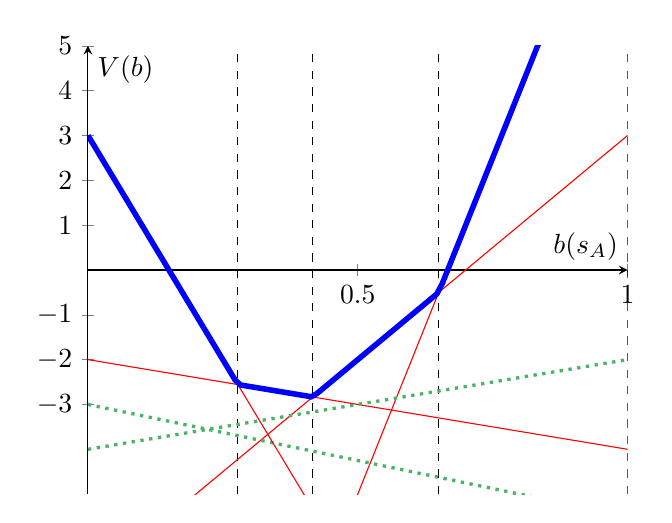
\begin{tikzpicture}[
  declare function={
    global(\x)= (\x>=(13/20)) * (30*\x-20) +
 and(\x>(5/12),\x<(13/20)) * (10*\x-7) +
 and(\x>(5/18),\x<=(5/12)) * ((-2)*\x-2) +
 and(\x>0,\x<(5/18)) * ((-20)*\x+3) +
 (\x<=0) * (3);
	alpha0(\x)= (30*\x-20);
	alpha1(\x)= (10*\x-7);
	alpha2(\x)= ((-2)*\x-2);
	alphabad1(\x)= ((-2.5)*\x-3);
	alphabad2(\x)= (2*\x-4);
	alpha3(\x)= ((-20)*\x+3);
  }
]
\begin{axis}[samples=100,
  axis x line=middle, axis y line=middle,
  ymin=-5, ymax=5, ytick={-3,-2,-1,0.0,...,10}, ylabel=$V(b)$,
  xmin=0, xmax=1, xtick={0,0.5,1}, xlabel=$b(s_A)$,
]

\pgfplotsinvokeforeach{5/18,5/12, 13/20, 1}{
  \draw[dashed] ({rel axis cs: 0,0} -| {axis cs: #1, 0}) -- ({rel axis cs: 0,1} -| {axis cs: #1, 0});}

\definecolor{ggreen}{rgb}{0.3,0.7,0.4};
\addplot[red, domain=0:1, smooth]{alpha0(x)};
\addplot[red, domain=0:1, smooth]{alpha1(x)};
\addplot[red, domain=0:1, smooth]{alpha2(x)};
\addplot[ggreen, domain=0:1, smooth, dotted, very thick]{alphabad1(x)};
\addplot[ggreen, domain=0:1, smooth, dotted, very thick]{alphabad2(x)};
\addplot[red, domain=0:1, smooth]{alpha3(x)};
\addplot[blue, domain=0:1, line width=2pt]{global(x)};
\end{axis}
\end{tikzpicture} 
\caption[Value function PWLC and $\alpha$-vectors for a state space $\mathcal{S} = \set{s_A,s_B}$]{Example of useful alpha vectors (red), value function PWLC (thick blue), and useless (bad) alpha vectors (dotted green) of a POMDP at a given iteration: 
the state space is $\mathcal{S} = \set{s_A,s_B}$: $x$-axis represents $b(s_A)$ 
and $y$-axis represents $V(b)$. As $\# \mathcal{S} = 2$, $b(s_B) = 1 - b(s_A)$.}  \label{alphavectors_POMDP} 
\end{figure}

\begin{figure}  
\center
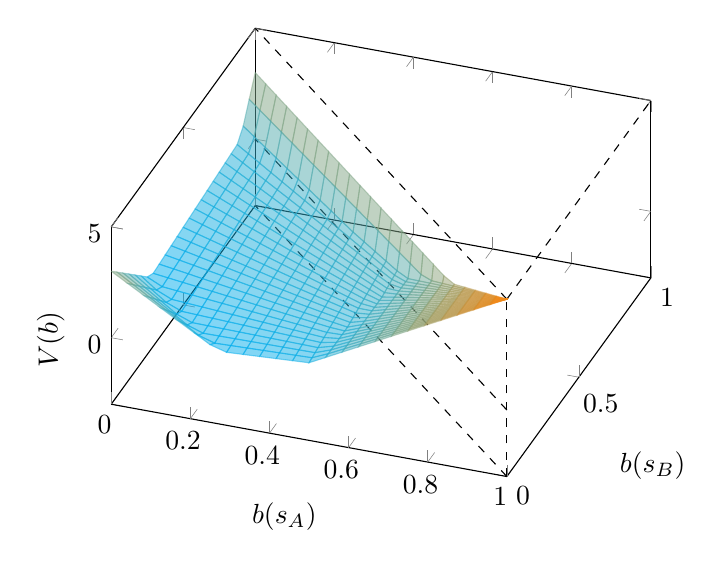
\begin{tikzpicture}[declare function={ 
		   deffun(\x,\y) = (\x+\y<=1);
		   nondeffun(\x,\y) = -10*(\x+\y>1);
                   myfun(\x,\y)  = 9*\x-7;
                   myfun2(\x,\y)  = 6*\y-4;
                   myfun3(\x,\y)  = 3*\y+4*\x-2;
		   myfun4(\x,\y)  = -5*\y-4*\x+3;
		   myfun5(\x,\y) = 5*\y-5*\x-2;
		   myfun6(\x,\y) = max(max(max( max(myfun(\x,\y), myfun2(\x,\y)), myfun3(\x,\y)),myfun4(\x,\y)),myfun5(\x,\y)) * deffun(\x,\y) + nondeffun(\x,\y);
                 },
]
\begin{axis}[xlabel=$b(s_A)$,ylabel=$b(s_B)$,zlabel=$V(b)$,view={20}{50},zmin=-3,zmax=5,
      variable=\s,variable y=\t,domain=0:1,
      colormap={custom}{color(0)=(cyan) color(1)=(orange)}]

\def\triangleParamX{\s}
\def\triangleParamY{(1-\s)*\t}

\def\myfun{9*\s-4};
\def\myfunTwo{20*\t-17};
\def\maxOneTwo{max(\myfun,\myfunTwo)};
\def\myfunThree{\t+\s};
\def\myfunFour{-10*\t-10*\s+3};
\def\maxThreeFour{max(\myfunThree,\myfunFour)};
\def\maxMaxMax{max(\maxOneTwo,\maxThreeFour)};


\addplot3[black,dashed] coordinates {(1,0,-3) (0,1,-3)};
\addplot3[black,dashed] coordinates {(1,0,0) (0,1,0)};
\addplot3[black,dashed] coordinates {(1,0,5) (0,1,5)};
\addplot3[black,dashed] coordinates {(1,0,-3) (1,0,5)};
\addplot3[black,dashed] coordinates {(1,0,5) (1,1,5)};
\addplot3[opacity=0.5,surf,shader=flat] (\triangleParamX,\triangleParamY,\maxMaxMax);


\end{axis}
\end{tikzpicture}
\caption[Value function PWLC for a state space $\mathcal{S} = \set{s_A,s_B,s_C}$]{
Value function PWLC at a given iteration when the state space is $\mathcal{S} = \set{s_A,s_B,s_C}$: $x$-axis represents $b(s_A)$, $y$-axis represents $b(s_B)$ 
and $z$-axis represents $V(b)$. As $\# \mathcal{S} = 3$, $b(s_C) = 1 - b(s_A) - b(s_B)$. $V(b)$ is the maximum of a set of hyperplans.}  \label{alphavectors_POMDP3D}  
\end{figure}

Given the number of iterations $N$ 
for a specified error bound $\varepsilon>0$ 
(see the error analysis of Section \ref{resMDP}), 
Algorithm \ref{algorithmIVPOMDP}
leads to a value function in the form of a set of $\alpha$-vectors $\Gamma_{\varepsilon}$:
$V^{\varepsilon}(b) = \max_{\alpha \in \Gamma_{\varepsilon}} \sum_{s \in \mathcal{S}} \alpha(s) \cdot b(s)$.
The associated strategy, approximately optimal, is 
\begin{align*}
 d^{\varepsilon}(b) & \in \operatorname*{argmax}_{a \in \mathcal{A}} \max_{ (\alpha_o) \in (\Gamma_{\varepsilon})^{\mathcal{O}}} \langle \alpha_{a,(\alpha_o)}, b \rangle_{\mathbb{R}^{\mathcal{S}}} \\
& \in \operatorname*{argmax}_{a \in \mathcal{A}} \max_{ (\alpha_o) \in \Gamma_{\varepsilon}^{\mathcal{O}}} \sum_{s \in \mathcal{S}} r(s,a) + \gamma \cdot \sum_{o' \in \mathcal{O}} \sum_{s' \in \mathcal{S}} \textbf{p} \paren{o' \sachant s',a} \cdot \textbf{p} \paren{ s' \sachant s ,a  } \cdot \alpha_{o'}(s').
\end{align*}
At execution, if the agent has a belief $b$,
and the $\alpha$-vector $\alpha_{a,(\alpha_o)}$ 
is such that $\forall \alpha \in \Gamma_{\varepsilon}$, $\langle \alpha_{a,(\alpha_o)}, b \rangle_{\mathbb{R}^{\mathcal{S}}} \leqslant \langle \alpha , b \rangle_{\mathbb{R}^{\mathcal{S}}}$,
then action $a$ is approximately optimal (with error $\varepsilon$).

\begin{algorithm} \caption{Value Iteration Algorithm for POMDP} 
\label{algorithmIVPOMDP}
$\Gamma \gets \Gamma^0$; \\
$i \gets 1$; \\
\While{$i \leqslant N$}{
	\For {$a \in \mathcal{A}$, $(\alpha_{o'}) \in \Gamma^{\mathcal{O}}$}{
		\For {$s \in \mathcal{S}$}{
			$\displaystyle \alpha(s) \gets r(s,a) + \gamma \cdot \sum_{o' \in \mathcal{O}} \sum_{s' \in \mathcal{S}} \textbf{p} \paren{o' \sachant s',a} \cdot \textbf{p} \paren{ s' \sachant s ,a  } \cdot \alpha_{o'}(s')$;
		}
	$ \Gamma' \gets \set{ \Gamma', \alpha }$;	
	}
$\Gamma \gets \Gamma'$;\\
$i++$;
}
\Return $\Gamma$;
\end{algorithm}

This algorithm is really naive since the number of $\alpha$-vectors 
increases as a double exponential with iterations: if $\forall n \in \mathbb{N}$, 
$\Gamma^n$ is the set of $\alpha$-vectors 
at the end of iteration $n$, and $g_n = \# \Gamma^n$, 
then $g_{n+1}=\# \mathcal{A} \cdot g_{n}^{\#\mathcal{O}}$. 
Thus, as $\# \mathcal{A}$ is the initial number of $\alpha$-vectors,
$g_n = (\# \mathcal{A})^{\sum_{i=0}^{n-1} (\# \mathcal{O})^i} \cdot (\# \mathcal{A})^{(\# \mathcal{O})^n}$

A first improvement consists in removing, 
at each iteration $i=1,\ldots,N$, 
dominated $\alpha$-vectors $\alpha_{bad} \in \Gamma^i$,
\textit{i.e.} $\alpha$-vectors such that 
$\max_{\alpha} \sum_{s \in \mathcal{S}} \alpha(s) \cdot b(s) > \sum_{s \in \mathcal{S}} \alpha_{bad}(s) \cdot b(s)$, 
$\forall b \in \mathbb{P}^{\mathcal{S}}$: 
Cassandra's algorithms use linear programs 
to prune these dominated $\alpha$-vectors 
\cite{Cassandra:1994:AOP:199480.199520,Cassandra97incrementalpruning}.

Whereas the resolution of finite state MDPs (MDPs with $\# \mathcal{S} < \infty$) is a P-complete problem \cite{Papadimitriou:1987},
solving a finite horizon POMDP is PSPACE-hard \cite{Papadimitriou:1987}, 
and solving an infinite horizon POMDP is undecidable \cite{Madani:1999:UPP:315149.315395}.
These theoretical complexities are a faithful representation of the difficulty of
solving POMDPs in practice. Algorithm \ref{algorithmIVPOMDP} or 
Cassandra's improvements \cite{Cassandra:1994:AOP:199480.199520,Cassandra97incrementalpruning}
solve only really small POMDPs, \textit{i.e.} POMDPs with a few system states and observations.
For instance in the case of robotic mission problems, 
the number of system states may be quite big,
as well as the number of observations,
and classical computations are intractable:
other computation methods are necessary to compute efficiently
a satisfactory strategy. The next section is devoted to the presentation
of the most notorious algorithms producing approximate stategies
within reasonable time.

\subsection{Computation of Strategies in Practice}
\label{section_SAalgo}
This section is meant to sum up the main ways 
to approximate POMDP optimal strategies,
as strategy computation is a difficult task in practice
and theoretically intractable
\cite{Papadimitriou:1987,Madani:1999:UPP:315149.315395}.

First consider $\widehat{V}$ and $\tilde{V}$
two functions mapping the set of all probability distributions 
$\mathbb{P}^{\mathcal{S}}$ to $\mathbb{R}$.
Suppose that $\forall b \in \mathbb{P}^{\mathcal{S}}$, 
$\widehat{V}(b) \leqslant \tilde{V}(b)$.
Then, $\forall b \in \mathbb{P}^{\mathcal{S}}$, 
\[ \Big(\mathcal{B}^* \widehat{V} \Big) (b) = \max_{a \in \mathcal{A}} \Big\{ \sum_{s \in \mathcal{S}} r(s,a) \cdot b(s) + \gamma \cdot \sum_{o' \in \mathcal{O}} \textbf{p} \paren{o' \sachant b , a } \cdot \widehat{V} \paren{ u(b,a,o')  } \Big\} \leqslant \Big( \mathcal{B}^* \tilde{V} \Big)(b) . \]
Thus, if $\forall b \in \mathbb{P}^{\mathcal{S}}$, $V(b) \leqslant V^*(b)$,
\textit{i.e.} if $V$ is a lower bound of the optimal value function $V^*$,
$\forall b \in \mathbb{P}^{\mathcal{S}}$,
$\Big( \mathcal{B}^* V \Big) (b) \leqslant \Big( \mathcal{B}^* V^* \Big) (b) = V^*(b)$.
As well, if $V$ is an upper bound of the optimal value function,
$\forall b \in \mathbb{P}^{\mathcal{S}}$,
$\Big( \mathcal{B}^* V \Big) (b) \geqslant \Big( \mathcal{B}^* V^* \Big) (b) = V^*(b)$.
This means that the iterations of the Dynamic Programming operator $\mathcal{B}^*$
on a lower (resp. upper) bound of $V^*$ return a lower (resp. upper)
bound of $V^*$.

Defining $r_{min} = \min_{s \in \mathcal{S}, a \in \mathcal{A}} r(s,a)$, 
the constant function $\underline{V_0}(b) = \sum_{t \geqslant 0} \gamma^t \cdot r_{min} = \frac{r_{min}}{1 - \gamma }$,
$\forall b \in \mathbb{P}^{\mathcal{S}}$,
is an example of initial lower bound 
of the optimal value function:
the worst reward is gathered at each time step.
The only $\alpha$-vector
representing this function is 
$\alpha_0(s) = \frac{r_{min}}{1 - \gamma }$, $\forall s \in \mathcal{S}$.

Let us start from an initial set of $\alpha$-vectors 
denoted by $\underline{\Gamma_0}$, defining a lower bound of the optimal value function,
\textit{i.e.} such that $\underline{V_0}(b) 
= \max_{\alpha \in \underline{\Gamma_0}} \sum_{s \in \mathcal{S}} \alpha(s) \cdot b(s) \leqslant V^*(b)$: 
for instance $\underline{\Gamma_0} = \set{ \alpha_0 }$. 
The $\alpha$-vectors $\alpha \in \underline{\Gamma_1}$ computed using the 
current $\alpha$-vector set $\Gamma_0$
and the equation (\ref{alpha_vector}) of Theorem \ref{PWLC_theorem},
take part in the definition of $\underline{V_1}(b) = \Big( \mathcal{B}^* \underline{V_0} \Big)(b)$.
As noted above, $\underline{V_1}$ is also a lower bound: $\underline{V_1}(b) 
= \max_{\alpha \in \underline{\Gamma_1}} \sum_{s \in \mathcal{S}} \alpha(s) \cdot b(s) 
= \Big( \mathcal{B}^* \underline{V_0} \Big) (b) \leqslant V^*(b)$, 
$\forall b \in \mathbb{P}^{\mathcal{S}}$.
Thus, as $\underline{V_0}$ and $\underline{V_1}$
are lower bounds of $V^*$, $\max \set{\underline{V_0}, \underline{V_1}}$ too,
\textit{i.e.} $\max_{\alpha \in \underline{\Gamma_0} \cup \underline{\Gamma_1}} \sum_{s \in \mathcal{S}} \alpha(s) \cdot b(s)$
is a lower bound of $V^*(b)$, and the best available at the moment.
Hence, it is sufficient to maintain a set of $\alpha$-vectors $\underline{\Gamma}$:
the $\alpha$-vectors computed from $\underline{\Gamma}$ may be added into $\underline{\Gamma}$, 
and the dominated ones may be removed.
Thanks to the convergence of $\Big( (\mathcal{B}^*)^n \underline{V_0} \Big)_{n \in \mathbb{N}}$ towards $V^*$, 
the computation of new $\alpha$-vectors tends to improve the lower bound.

The presented mechanism of incremental improvement
of the lower bound of $V^*$
using new $\alpha$-vectors 
does not allow to compute an upper bound:
starting from an upper bound $\overline{V_0}$,
if the computed $\alpha$-vectors represent
a function $\overline{V_1}$ (also an upper bound of $V^*$)
which tends to be closer to $V^*$ than $\overline{V_0}$ (thanks to the convergence), 
then $\max \set{ \overline{V_0}, \overline{V_1}  }$
is not a better upper bound: it is actually the worst.

Another method can be used to maintain and improve an upper bound 
of the value function: 
an upper bound $\overline{V}_0$ of the optimal value function is only
computed over a set of $n>0$ beliefs,
leading to the belief-value mappings 
$\set{ b_i, \overline{v}_i }_{i=1}^{n}$,
where $\overline{V}_0(b_i) = \overline{v}_i$
and $(b_i,v_i) \in \mathbb{P}^{\mathcal{S}} \times \mathbb{R}$.
As the limit of a sequence of convex functions
is convex, the optimal value function $V^*$ is known to be convex.
As the mappings are such that $v_i \geqslant V^*(b_i)$, 
and as $V^*$ is convex, any convex combination of the beliefs $(b_i)_{i=1}^n$
has an optimal value lower or equal to the same convex combination of the upper bound values $(\overline{v_i})_{i=1}^n$.
Indeed, if $(w_i)_{i=1}^n$ are convex coefficients, \textit{i.e.} 
$\sum_{i=1}^n w_i = 1$ and $\forall i \in \set{1,\ldots,n}$, $w_i\geqslant 0$,
then the optimal value function at $\sum_{i=1}^n w_i \cdot b_i$ 
is bounded by the convex combination of $(\overline{v_i})_{i=1}^n$
with respect to $(w_i)_{i=1}^n$: $V^*(\sum_{i=1}^n w_i \cdot b_i) \leqslant \sum_{i=1}^n w_i \cdot V^*(b_i) \leqslant \sum_{i=1}^n w_i \cdot \overline{v_i}$.
In order to get an upper bound of $V^*$ defined on a larger set of beliefs, 
the belief-value mappings $\set{ b_i, \overline{v_i} }_{i=1}^n$
may be completed with the couples $(b,v)$ such that
$b \in \mathbb{P}^{\mathcal{S}}$ is in the convex hull of $(b_i)_{i=1}^{n}$,
and $v$ is the lowest value of $\sum_{i=1}^n w_i \cdot \overline{v_i}$,
where $(w_i)_{i=1}^n$ convex coefficients such that $b = \sum_{i=1}^n w_i \cdot b_i$.
These coefficients defining the interpolation of the belief-value mappings 
can be computed using linear programming
or with approximate computations 
\cite{DBLP:journals/corr/abs-1106-0234,conf/aips/PoupartKK11}.
Finally, consider $b_j \in (b_i)_{i=1}^n$ 
such that $\forall a \in \mathcal{A}$, $\forall o' \in \mathcal{O}$,
$u(b_j,a,o')$ is in $(b_i)_{i=1}^n$.
The upper bound value $\overline{v_j}$ associated to $b_j$ can be replaced by 
$(\mathcal{B}^* \overline{V}_0)(b_j)$, computed using the equation (\ref{equation_bellmanOperator_POMDP}) defining the Dynamic Programming operator $\mathcal{B}^*$:
\[ (\mathcal{B}^* \overline{V}_0)(b_j) = \max_{a \in \mathcal{A}} \Big\{ \sum_{s \in \mathcal{S}} r(s,a) \cdot b_j(s) + \gamma \cdot \sum_{o' \in \mathcal{O}} \textbf{p} \paren{o' \sachant b_j , a } \overline{V}_0 \paren{ u(b_j,a,o')  } \Big\}, \]
where $\overline{V}_0 \paren{ u(b_j,a,o')  } = \overline{v_k}$
with $u(b_j,a,o') = b_k \in (b_i)_{i=1}^n$.
This value update replaces then the value $\overline{v_j}$
and leads to an improved upper bound of the optimal value function in $b_j$.
A famous and simple method to compute an initial upper bound of $V^*$ 
is called the $Q_{MDP}$ method \cite{Littman96algorithmsfor}: 
it consists in computing an optimal value function
for the underlying MDP \textit{i.e.} for the MDP built 
ignoring the observations and the observation probabilities, 
and considering that the state is fully observable.
A MDP strategy is looked for among a more general set of functions 
of the data available at execution, 
than a POMDP strategy. 
First, the reward is defined on the system states and the actions,
which are directly available during execution in fully observable settings. 
Second, as the uncertainty over the observations is conditional on the system state,
the observation random variables $O_t$ can be written as measurable functions of the state and action variables $S_t$ and $A_{t-1}$:
the functions from the actions and the observations consist thus of a subset of the functions from the system states and the actions.
We can conclude that, the optimal value function of the POMDP starting from the deterministic belief $b^A_0(s) = \mathds{1}_{ \set{s=s_A}}$ with $s_A \in \mathcal{S}$,
namely 
\[ V^*(b^A_0) = \max_{  \substack{ (d_t)_{t \geqslant 0} \mbox{ \tiny s.t. } \\ d_t: \mathcal{I}_t \rightarrow \mathcal{A}  }} \mathbb{E}_{S_0 \sim b^A_0} \croch{ \sum_{t \geqslant 0} \gamma^t \cdot r\Big(S_t,d(I_t)\Big) }, \]
is lower or equal to the optimal value function for the associated MDP starting from $s_A$: 
\[ V_{MDP}^*(s_A) = \max_{  \substack{ (d_t)_{t \geqslant 0} \mbox{ \tiny s.t. } \\ d_t: \mathcal{S} \rightarrow \mathcal{A} } } \mathbb{E} \croch{ \sum_{t \geqslant 0} \gamma^t \cdot r\Big(S_t,d(S_t)\Big) \sachant S_0 = s_A  }. \]
Indeed, the maximum operator of the latter 
is performed on a set of functions including 
the one used to maximize the POMDP value function at $b^A_0$ (first equation).
Hence, an initial upper bound of the POMDP optimal value function $V^*$ can be computed for the deterministic beliefs \textit{i.e.} 
the beliefs $b \in \mathbb{P}^{\mathcal{S}}$ such that $b(s) = \mathds{1}_{\set{ s=s_A }}$ with $s_A \in \mathcal{S}$:
$\overline{V_0}(b) \geqslant V_{MDP}^*(s_A)$. 
The convex hull of these deterministic beliefs is the full set of probability distributions $\mathbb{P}^{\mathcal{S}}$.
Thus, using the previous interpolation trick, an upper bound of $V^*$ is available in the full belief space $\mathbb{P}^{\mathcal{S}}$. 
Other methods to compute bounds for $V^*$ are available for instance in \cite{conf/aaai/Hauskrecht97}.

\begin{figure} 
\center
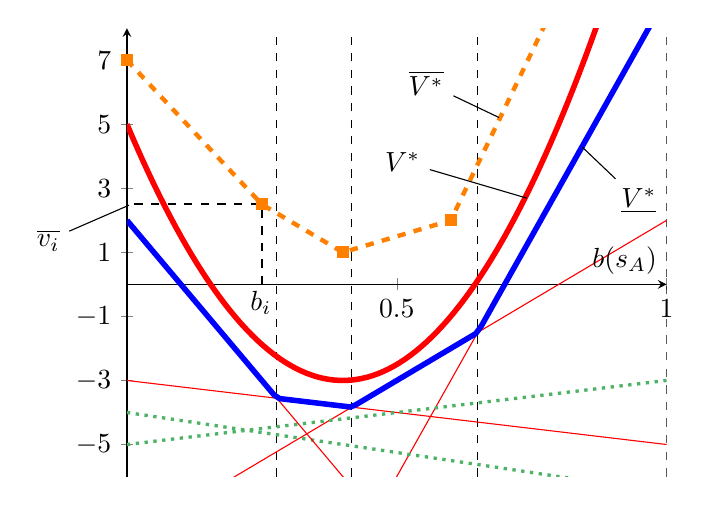
\begin{tikzpicture}[
  declare function={
    global(\x)= (\x>=(13/20)) * (30*\x-21) +
 and(\x>(5/12),\x<(13/20)) * (10*\x-8) +
 and(\x>(5/18),\x<=(5/12)) * ((-2)*\x-3) +
 and(\x>0,\x<(5/18)) * ((-20)*\x+2) +
 (\x<=0) * (2);
	alpha0(\x)= (30*\x-21);
	alpha1(\x)= (10*\x-8);
	alpha2(\x)= ((-2)*\x-3);
	alphabad1(\x)= ((-2.5)*\x-4);
	alphabad2(\x)= (2*\x-5);
	alpha3(\x)= ((-20)*\x+2);
	valuefunction(\x) = (50*(\x-0.4)*(\x-0.4) -3);
  }
]
\begin{axis}[samples=100,
  axis x line=middle, axis y line=middle,
  ymin=-6, ymax=8, ytick={-5,-3,-1,...,7},
  xmin=0, xmax=1, xtick={0,0.5,1}, xlabel=$b(s_A)$,
]

\pgfplotsinvokeforeach{5/18,5/12, 13/20, 1}{
  \draw[dashed] ({rel axis cs: 0,0} -| {axis cs: #1, 0}) -- ({rel axis cs: 0,1} -| {axis cs: #1, 0});}

\definecolor{ggreen}{rgb}{0.3,0.7,0.4};
\addplot[red, domain=0:1, smooth]{alpha0(x)};
\addplot[red, domain=0:1, smooth]{alpha1(x)};
\addplot[red, domain=0:1, smooth]{alpha2(x)};
\addplot[ggreen, domain=0:1, smooth, dotted, very thick]{alphabad1(x)};
\addplot[ggreen, domain=0:1, smooth, dotted, very thick]{alphabad2(x)};
\addplot[red, domain=0:1, smooth]{alpha3(x)};
\addplot[blue, domain=0:1, line width=2pt]{global(x)};
\addplot[red, domain=0:1, line width=2pt]{valuefunction(x)};
\addplot[orange, ultra thick, dashed] coordinates { (0, 7) (0.25, 2.5) (0.4, 1) (0.6, 2) (0.8,9)  };
\addplot[orange, mark=square*,only marks] coordinates { (0, 7) (0.25, 2.5) (0.4, 1) (0.6, 2) (0.8,9)  };
\addplot[dashed, thick] coordinates { (0.25, 0) (0.25, 2.5) (0, 2.5)};
\end{axis}
\node (optvalue) at (3.5,4) {$V^*$};
\node (optvaluecurve) at (5.2,3.5) {};
\draw (optvalue) -- (optvaluecurve);

\node (upper) at (3.8,5) {$\overline{V^*}$};
\node (uppercurve) at (4.85,4.5) {};
\draw (upper) -- (uppercurve);

\node (lower) at (6.5,3.5) {$\underline{V^*}$};
\node (lowercurve) at (5.66,4.3) {};
\draw (lower) -- (lowercurve);

\node (bi) at (1.7,2.2) {$b_i$};
\node (vi) at (-1,3) {$\overline{v_i}$};
\node (vicurve) at (0.15,3.5) {};
\draw (vi) -- (vicurve);
\end{tikzpicture} 
\caption[Bounds of the optimal Value function $V^*$
used to approximate it]{Bounds of the optimal value function $V^*$. 
The latter is represented by the regular thick red line.
The lower bound $\underline{V^*}$ is the piecewise linear function represented by the thick blue line.
Useful $\alpha$-vectors are represented by the thin red lines,
and dominated ones are represented by dotted green lines.
The upper bound $\overline{V^*}$ is represented by the piecewise linear dashed orange line: 
the squares represent the belief-value mappings. }  \label{bounds_POMDP} 
\end{figure}

Some recent POMDP solvers are said to be \textit{point-based} as they maintain
a set of beliefs $(b_i)_{i=1}^n$ (the \textit{belief points}) 
and the associated $\alpha$-vectors $\alpha$-vectors $(\alpha_i)_{i=1}^n$.
The current approximation $V$ of the optimal value function is described 
by $(\alpha_i)_{i=1}^n$: $\forall b \in \mathbb{P}^{\mathcal{S}}$,
$V(b) = \max_{i=1}^n \sum_{s \in \mathcal{S}} \alpha_i(s) \cdot b(s)$. 
Each belief of $(b_i)_{i=1}^n$ is such that
$V(b_i) = \sum_{s \in \mathcal{S}} b_i(s) \cdot \alpha_i(s)$.
The point-based Bellman backup of a belief $b_i$ is the replacement of its $\alpha$-vector 
$\alpha_i$ by one of the new $\alpha$-vectors (Equation \ref{alpha_vector}) 
which maximize the equation (\ref{bellman_alpha}) 
with the belief $b_i$, \textit{i.e.} replacing it by 
$\alpha' \in \operatorname*{argmax}_{\alpha' \in \Gamma'} \langle \alpha', b_i \rangle_{\mathbb{R}^{\mathcal{S}}}$.

The first point-based algorithm was PBVI (\textit{Point-Based Value Iteration})
\cite{Pineau_2003_4826} which starts with a single belief point $b_0$.
At a given iteration, the point-based Bellman backup of each belief 
of the current set $(b_i)_{i=1}^n$ are computed and lead to a new set of 
$\alpha$-vectors $(v_i')_{i=1}^n$. This operation is repeted until
the convergence of the $\alpha$-vectors. Next, for each belief in $(b_i)_{i=1}^n$,
one successor is selected: the most distant one from $(b_i)_{i=1}^n$, 
with respect to a given distance metric.
These successors are added to the set, which becomes $(b_i)_{i=1}^{2n}$,
and the next iteration begins.

Another point-based POMDP solver is the \textit{Perseus} solver \cite{Spaan04techrep}:
this solver starts running trials of random exploration of the belief space,
sampling $a \in \mathcal{A}$ and observation $o' \in \mathcal{O}$ at each time step of a trial 
to compute the next belief $b'=u(b,a,o')$ from the current one $b \in \mathbb{P}^{\mathcal{S}}$.
The set of all reached beliefs is $(b_i)_{i=1}^{n}$ and does not evolve anymore. 
A lower bound PWLC $\underline{V}$ is used to approach the value function:
the associated set of $\alpha$-vectors is denoted by $\underline{\Gamma}$.
At each iteration, $\mathbb{B}$ is initialized as a copy of $(b_i)_{i=1}^{n}$,
and $\Gamma = \emptyset$. 
While $\mathbb{B} \neq \emptyset$, an arbirary belief $b$ is selected in $\mathbb{B}$,
and the associated new $\alpha$-vector $\alpha'$ is computed with the point-based Bellman backup on $b$ 
and using $\underline{\Gamma}$.
If $\langle \alpha', b \rangle_{\mathbb{R}^{\mathcal{S}}} \geqslant \underline{V}(b)$,
all the beliefs whose value is improved by $\alpha'$,
\textit{i.e.} the beliefs $\tilde{b} \in \mathbb{B}$ such that
$\langle \alpha', \tilde{b} \rangle_{\mathbb{R}^{\mathcal{S}}} \geqslant \underline{V}(\tilde{b}) $, are removed from $\mathbb{B}$.
The new $\alpha'$ is added to $\Gamma$.
Otherwise, if $\langle \alpha', b \rangle_{\mathbb{R}^{\mathcal{S}}} < \underline{V}(b)$,
$b$ is removed from $\mathbb{B}$ and an $\alpha$-vector from 
$\underline{\Gamma}$ $\tilde{\alpha} \in \operatorname*{argmax}_{\alpha \in \underline{\Gamma}} \langle \alpha, b \rangle_{\mathbb{R}^{\mathcal{S}}}$ 
is added into $\Gamma$. When $\mathbb{B} = \emptyset$, $\underline{\Gamma}$ is set to $\Gamma$,
and a new iteration begins.

The HSVI solver (\textit{Heuristic Search Value Iteration}) \cite{Smith:2004:HSV:1036843.1036906} is also a point-based algorithm.
This solver maintains both an upper and a lower bound of $V^*$: $\overline{V}$ and $\underline{V}$.
It takes into account that the error of the approximation of $V^*$ 
is less important for much later successors of $b_0 \in \mathbb{P}^{\mathcal{S}}$,
due to the discount factor $\gamma$:
given an error $\varepsilon>0$, a sequence of beliefs $(b_t)_{t\geqslant0}$ is generated
from $b_0$ until $\overline{V}(b_t) - \underline{V}(b_t) < \frac{\varepsilon}{\gamma^t}$. 
The generation of the belief sequence is done selecting actions 
according to the upper bound: if the current belief is $b$, the chosen action is in
$\operatorname*{argmax}_{a \in \mathcal{A}} r(s,a) + \gamma \sum_{o' \in \mathcal{O}} \overline{V}\Big(u(b,a,o')\Big)$.
This trick tends to force the improvement of the upper bound: if the selected action is not optimal,
as successors for this action are selected, the computations will focussed on
these beliefs, and will decrease (improve) the upper bound for them.
As well, the observation selected $o' \in \mathcal{O}$ is such that 
the value $\overline{V}\Big(u(b,a,o')\Big) - \underline{V}\Big(u(b,a,o')\Big) \cdot \textbf{p} \paren{ o' \sachant b, a }$ is the greatest:
the probable beliefs for which $\overline{V}$ and $\underline{V}$
are poor bounds are preferred, in order to focus the computational efforts
on the belief space subsets where the bounds are the worst. 
Then, both bounds are updated starting with the last reached belief
back in time step to $b_0$: this order makes these updates more efficient.
The scheme starting with a belief sequence generation, and updating the bounds on it,
is repeated until $\overline{V}(b_0) - \underline{V}(b_0) < \varepsilon$.

The solver SARSOP \cite{Kurniawati-RSS08}, inspired by HSVI and FSVI \cite{shani}, 
refines the generation method of the belief sequence. 
First of all, the belief space is clustered using a simple learning technique:
the features are for intance the initial upper bound 
$\underline{V_0}$ and the entropy of beliefs.
This discretization is used to maintain an estimation of the optimal value function denoted by $\widehat{V}$:
this estimation is constant over each cluster, equal to 
the average of the estimated optimal value of the beliefs in this cluster.
Let $b$ be a belief reached during a generation of a belief sequence:
$L_1$ is real number such that $L_1 \leqslant V^*(b)$.
Let $L_2 = \Big( \mathcal{B}^* \underline{V} \Big)(b)$. 
Thus, the lower bound of the optimal value function $\underline{V}$ on $b$
is likely to be improved by selecting the next belief $b'=u(b,a,o')$ 
(where $a \in \mathcal{A}$ and $o' \in \mathcal{O}$ are selected as in HSVI)
if the optimal value of $b'$ is likely to be big enough for it:
that is, if $r(b,a) + \gamma \cdot \bigg( \textbf{p} \paren{ o' \sachant b,a } \cdot \widehat{V}(b') + \sum_{\tilde{o} \neq o'} \textbf{p} \paren{ \tilde{o} \sachant b,a } \cdot \underline{V}\Big(u(b,a,\tilde{o})\Big) \bigg)$ is greater than $L = \max \set{ L_1, L_2 }$.
In this case, if $L_1'$ such that $L = r(b,a) + \gamma \cdot \bigg( \textbf{p} \paren{ o' \sachant b,a } \cdot L_1' + \sum_{\tilde{o} \neq o'} \textbf{p} \paren{ \tilde{o} \sachant b,a } \cdot \underline{V}\Big(u(b,a,\tilde{o})\Big) \bigg)$, 
the condition $\widehat{V}\Big(u(b,a,\tilde{o})\Big) \geqslant L_1'$ 
is a good indicator that the selection of the belief $b'$ is likely to improve the current lower bound at $b$:
if $\widehat{V}(b') \geqslant L_1'$ (and if, as in HSVI, $\overline{V}(b') - \underline{V}(b') \leqslant \frac{\varepsilon}{\gamma^t}$), 
the belief $b'$ is selected and the same test is performed on its successor knowing that $V^*(b')$ is likely to be greater than $L_1'$.
In this way, the belief sequences selected may be longer than in HSVI,
as sequence generation continues if the next beliefs are likely to improve optimal value function estimation. 
Next, when the generation of the sequence ends, 
the bound updates start from the last belief to $b_0$, 
following the generated belief sequence
in the reverse order (as with HSVI).
Finally, SARSOP proposes also another major computation simplification:
all the previous belief sequence generations can be summed up  
in a tree representing the different transitions $b \rightarrow u(b,a,o')$
and which is recorded in the memory. 
Let us define $\underline{Q}(b,a) = r(b,a) + \gamma \cdot \sum_{o' \in \mathcal{O}} \textbf{p} \paren{ o' \sachant b,a } \cdot \underline{V}\Big( u \paren{ b,a,o' } \Big)$,
and $\overline{Q}(b,a)$ with the same formula replacing  $\underline{V}$ by $ \overline{V}$.
If $b$ is a belief, $a$ an action, and 
$\exists a' \in \mathcal{A}$, $\exists b' \in \mathbb{P}^{\mathcal{S}}_{b_0}$ 
such that $\overline{Q}(b,a) \leqslant \underline{Q}(b',a')$,
then, all the successors of $b$ by selecting action $a$ are
removed from the three, and the associated $\alpha$-vectors deleted.
Indeed, less stored $\alpha$-vectors and beliefs speed up the POMDP resolution,
as lots of useless computations are avoided:
the computations are focused on the beliefs which seems to be in $\mathbb{P}^{\mathcal{S}}_{b_0,*}$,
the notation for the subset of $\mathbb{P}^{\mathcal{S}}_{b_0}$
containing the beliefs reached with an optimal strategy.

While the $\alpha$-vector (or Sondic's) representation is used by a large part
of the POMDP solvers, the \textit{grid-based} POMDP solvers, which does not use it, 
are also popular algorithms \cite{bonet:icml02,Lovejoy91,Brafman97aheuristic,Bonet_newgrid-based}.
These solvers are based on a discretization of the belief space $\mathbb{P}^{\mathcal{S}}$
which leads to an MDP over the finite set of discretized beliefs: 
computed strategies map any cluster of beliefs to an action $a \in \mathcal{A}$.

Another POMDP solver based on a discretization of the belief space is RTDP-bel \cite{Geffner98solvinglarge}.
The discretization is only used to store a finite number of values during the computations.
The approximation maintains the approximate optimal value function as a piecewise constant function:
two beliefs in the same discretization group have the same value.
The algorithm operates in the same way as RTDP (\textit{Real Time Dynamic Programming}) \cite{Barto93learningto},
a \textit{Goal-MDP} solver which converges to the optimal value function without considering all the system states.
A Goal-MDP \cite{Bertsekas:2000:DPO:517430} is an MDP 
whose all rewards are negative and with a subset of the system state $\mathcal{G} \subset \mathcal{S}$
called \textit{set of goals}. The system states in $\mathcal{G}$ are absorbing and cost-free: 
$\forall (s,a) \in \mathcal{G} \times \mathcal{A}$,
$r(s,a)=0$ and $\textbf{p} \paren{s \sachant s,a} = 1$.
The criterion of a Goal-MDP is the expected (undiscounted) total reward,
\textit{i.e.} the expectation of the sum of the rewards over time steps (without factors $\gamma^t$).
As well, a \textit{Goal-POMDP} is a POMDP with only negative rewards
and a set of goals $\mathcal{G}$ which are  absorbing, cost-free and fully observable system states \textit{i.e.}
$\mathcal{O}$ contains $\mathcal{G}$ too, 
and $\forall s' \in \mathcal{G}$, $\forall a \in \mathcal{A}$, $\forall t \geqslant 0$,
$\mathbb{P} \paren{ O_{t+1} = s' \sachant S_{t+1} = s', a  } = 1$.
In fact RTDP-bel is a Goal-POMDP solver.
It initializes the value function $V$ with a (piecewise constant) upper bound called \textit{admissible heuristique}.
Then, the repetition of trials starting from $b_0$ improves the approximation of the optimal value function and the associated strategy.
At a given stage of a trial, the current belief is denoted by $b$. 
The $Q$-value is $Q(b,a) = \set{ r(b,a) + \sum_{o' \in \mathcal{O}} \textbf{p} \paren{ o' \sachant b, a  } \cdot V \Big( u(b,a,o') \Big) }$.
An action $a \in \operatorname*{argmax}_{\tilde{a} \mathcal{A}} Q(b,\tilde{a})$
is selected, and $V(b)$ is updated to $\max_{a \in \mathcal{A}} Q(b,a)$.
Then $s$ is sampled from $b$, as well as $s'$ according to $\textbf{p} \paren{ s' \sachant s,a }$, 
and $o'$ using $\textbf{p} \paren{ o' \sachant s',a }$.
If $b'=u(b,a,o')$ is such that $\forall s \in \mathcal{S}\setminus\mathcal{G}$, 
$b'(s)=0$, then another trial begins. Otherwise, the next stage of the trial consider $b'$.
Any classical (discounted) POMDP (Section \ref{section_definition_POMDP})
can be translated into a Goal-POMDP \cite{DBLP:conf/ijcai/BonetG09},
then RTDP-bel can solve any POMDP.

Finally, POMCP \cite{NIPS2010_4031} is the partially observable counterpart 
of the MDP solver UCT \cite{Kocsis:2006:BBM:2091602.2091633}. 
The latter is based on the UCB (Upper Confidence Bound) strategy for stochastic bandits \cite{Auer:2002:FAM:599614.599677}
and is an instance of MCTS (Monte-Carlo Tree Search) \cite{2008}.
A decision tree whose nodes are the reached states and arrows are the actions, 
is built during simulations to maintain at each node
the counts $N(s,a)$ of the visit of the couple $(s,a)$, $\forall a \in \mathcal{A}$.
The estimation $V$ of the optimal value function
is computed by Monte-Carlo simulations.
The $Q$-value is $Q(s,a) = \set{ r(s,a) + \gamma \cdot \sum_{s' \in \mathcal{S}} \textbf{p} \paren{ s' \sachant s,a } \cdot V(s') }$.
The UCB-inspired exploration-exploitation strategy is to select 
$a \in \operatorname*{argmax}_{a \in \mathcal{A}} \set{ Q(s,a)+ c \cdot \sqrt{ \frac{log N(s)}{N(s,a)} } }$, 
where $N(s) = \sum_{a \in \mathcal{A}} N(s,a)$ 
and $c>0$ is the relative ratio between exploration to exploitation: 
the more $c$ is small, the more actions with high values are selected (exploitation),
the more $c>0$ is big, the more the actions are selected with about the same rate,
without paying attention to the estimated values. 
The term $c \cdot \sqrt{ \frac{log N(s)}{N(s,a)} }$ is meant to
force the actions rarely tried before to be selected (exploration).
In the case of POMCP, during computations, the belief is approximated 
by an unweighted particule filter $B_t(s) \approx \frac{1}{K} \sum_{i=1}^{K} \mathds{1}_{S_i = s}$
where $\forall i=1,\ldots,K$, $S_i \sim B_t$, 
and the nodes of the tree represent possible successive information 
$i_t = \set{a_0,o_1,\ldots,a_{t-1},o_t}$, 
instead of the system states like in UCT.

The algorithms presented in this section 
are part of the state of the art POMDP solvers,
and some of them will be used in the next chapters
in order to propose comparisons with our work.
Now, the second main subject of this thesis
is presented: Possibility Theory, and the qualitative possibilistic counterpart
of the Partially Observable Markov Decision Processes.
